\chapter{Eficiência Energética}

%%%%%%%%%%%%%%%%%%%%%%%%%%%%%%%%%%%%%%%%%%%%%%%%%%%%%%%%%%%%%%%%%%%%%%%%%%%%%%
%%%%%%%%%%%%%%%%%%%%%%%%%%%%% Consumo de Energia %%%%%%%%%%%%%%%%%%%%%%%%%%%%%
%%%%%%%%%%%%%%%%%%%%%%%%%%%%%%%%%%%%%%%%%%%%%%%%%%%%%%%%%%%%%%%%%%%%%%%%%%%%%%

\section{Consumo de Energia}

\subsection{Consumo energético por habitante}

	De acordo com os dados coletados no Anuário Estatístico de Energia Elétrica de 2013, a média de consumo de uma residência no Distrito Federal, dos anos de 2008 à 2012, é de 217,72 \nicefrac{\si{\kilo\watt\hour}}{mês}, porém, esses dados não levam em consideração o tamanho da habitação ou a quantidade de moradores. Segundo o mesmo anuário, cada habitante gasta em média 2,1532 \nicefrac{\si{\kilo\watt\hour}}{dia} e em média 65\si{\kilo\watt\hour} mensal\cite{2013Aneel}.

\subsection{Consumo médio de uma família para 4 pessoas}

	Fazendo um cálculo meramente estatístico, numa estimativa grosseira, supondo um mês com 30 dias e 4 habitantes com a média de consumo idênticas, obtemos que o consumo médio de energia de uma residência com 4 pessoas sendo de 258,384 \nicefrac{\si{\kilo\watt\hour}}{mês}. Ainda de acordo com esses valores, pode-se supor que essa média não leva em consideração a classe social da família, onde, a grosso modo, sabe-se que quanto maior a renda familiar, maior serão os seus gastos. Como os equipamentos de segurança e outros objetos mais específicos voltados a automação e outros equipamentos que fogem do padrão residencial não foram bem detalhados, faz-se uma estimativa, ainda embasado no consumo médio residencial brasileiro, de que a família consumirá uma média de 500 \nicefrac{\si{\kilo\watt\hour}}{mês}.

\subsection{Horários de maior consumo}

	Composta por 4 moradores, baseado na média nacional, o modelo familiar ainda segue o padrão histórico, no caso, um casal com filhos. Ressaltando que não foram levados em consideração o conceito de família encontrado na legislação, portanto atribui-se o conceito de casal como a união entre homem e mulher baseando-se apenas nos dados do \cite{IBGE} quanto aos tipos de família. Para justificativas de cálculos e média de consumo da família, é importante que se estabeleça sua rotina, bem como as faixas etária de cada habitante. Ainda com base nos dados sobre a média etária da população, de acordo com o censo demográfico, estabeleceu-se que o casal tenha entre 30 – 44 anos, e os filhos, um entre 15 – 29 anos e o outro entre 0 – 14 anos.

	Sendo que, o casal trabalha em horário comercial e os filhos estão em idade escolar, permanecendo todos fora da casa durante o dia e se reunindo em casa no período noturno, a partir das 18h. Obedecendo assim os horários de consumo energético médio do país, onde os horários de consumo e de pico se fixam a partir das 18\si{\hour} até as 23\si{\hour} nos dias uteis.

\subsection{Fontes consumidoras}

	Abaixo encontra-se a tabela dos eletrodomésticos comuns usados pela família, baseado nos eletrodomésticos de uso comum encontrado na média das famílias brasileiras segundo dados da \cite{2013Aneel}, bem como dados referentes a potência de cada equipamento (dado encontrado pelas especificações do fabricante em cada aparelho), a quantidade de cada equipamento presenta na casa, o uso em horas por dia e a quantidade de dias num mês em que se usa cada aparelho, por fim têm-se a última coluna onde calcula-se o consumo mensal de cada aparelho e no fim o resultado do consumo médio mensal da residência. Para o cálculo de consumo médio não se levou em consideração os equipamentos de segurança, bem como sensores e câmeras de monitoramento, se tratando apenas de valores hipotéticos e apenas para fins estatísticos.

\begin{table}[H]
\noindent\begin{tabular}{|c|c|c|c|c|c|}
\hline
\textbf{Eletrodoméstico} & \textbf{Qte} & \textbf{Potência [\si{\watt}]} & \textbf{Uso Diário [\si{\hour}]} & \textbf{Qte dias/mês} & \textbf{[\si{\kilo\watt\hour}] Mensal}\tabularnewline
\hline
\hline
Ar condicionado & 4 & 1400 & 1 & 10 & 56\tabularnewline
\hline
Aspirador de pó & 1 & 600 & 1 & 5 & 3\tabularnewline
\hline
Batedeira & 1 & 100 & 1 & 4 & 0,4\tabularnewline
\hline
Computador & 1 & 300 & 1 & 30 & 9\tabularnewline
\hline
Fero Elétrico & 1 & 1000 & 2 & 4 & 8\tabularnewline
\hline
Fogão (cooktop) & 1 & 3000 & 1 & 26 & 78\tabularnewline
\hline
Forno Elétrico & 1 & 1500 & 1 & 12 & 18\tabularnewline
\hline
Freezer\parnote{} & 1 & 300 & 10 & 30 & 90\tabularnewline
\hline
Geladeira\parnote{O tempo médio de 10 horas diárias para geladeira e freezer refere-se ao período em que o compressor fica ligado para manter o interior na temperatura desejada\label{compressor}} & 1 & 115 & 10 & 30 & 34,5\tabularnewline
\hline
Home Theatre & 1 & 150 & 2 & 4 & 1,2\tabularnewline
\hline
Lâmpadas & 30 & 6 & 5 & 20 & 18\tabularnewline
\hline
Lava-louças & 1 & 1500 & 1 & 4 & 6\tabularnewline
\hline
Liquidificador & 1 & 200 & 0,5 & 10 & 1\tabularnewline
\hline
Máquina de lavar & 1 & 1000 & 2 & 5 & 10\tabularnewline
\hline
Microondas & 1 & 2000 & 0,5 & 15 & 15\tabularnewline
\hline
Notebook & 4 & 65 & 2 & 26 & 13,52\tabularnewline
\hline
Secador & 1 & 1000 & 0,5 & 30 & 15\tabularnewline
\hline
Televisão & 3 & 90 & 2 & 30 & 16,2\tabularnewline
\hline
Vídeo game & 1 & 20 & 2 & 15 & 0,6\tabularnewline
\hline
\multicolumn{5}{|c|}{\textbf{Consumo total mensal [\si{\kilo\watt\hour}/mes]}} & 393,42\tabularnewline
\hline
\end{tabular}
\parnotes
\caption{Consumo mensal dos eletrodomésticos}
\label{consumo_eletrodomesticos}
\end{table}

Para cálculo do consumo mensal foi utilizado a seguinte expressão:

\begin{equation*}
	C_m = \sum \dfrac{P * Q_a * U_d * Q_d}{1000}
\end{equation*}

Onde $P$ é a potência, valor encontrado nas especificações de cada aparelho dado em watts [\si{\watt}]. $Q_a$ é a quantidade de aparelhos, o número referente à quantidade de um mesmo aparelho presente na casa, valor adimensional. $U_d$ é o uso diário, tempo estimado em que o equipamento consome energia elétrica da casa por dia, valor em horas [\si{\hour}]. $Q_d$ é a quantidade de dias, o número de dias em que o equipamento é usado ligado à rede elétrica no período de um mês, sendo considerado um mês com 30 dias, valor adimensional. E por fim, $C_m$ é o consumo mensal, é a soma do consumo de todos os aparelhos durante o mês, valor em quilowatt-hora \nicefrac{\si{\kilo\watt\hour}}{mês}.

\subsection{Valor da tarifa referente à CEB}
	
	De acordo com a ANEEL, a CEB homologou uma tarifa de 0,43676 reais por quilowatt-hora (\nicefrac{R\$}{\si{\kilo\watt\hour}}).
Valores na tabela abaixo, disponibilizada pela ANEEL.

\begin{table}[H]
\centering
\begin{tabular}{|l|c|}
\hline 
\multicolumn{2}{|l|}{Empresa: CEB-DIS - CEB Distribuição S.A.}\tabularnewline
\hline 
\multicolumn{2}{|l|}{Vigência da Tarifa de 26/08/2015 a 25/08/2016}\tabularnewline
\hline 
\multicolumn{2}{|l|}{Resolução Homologatória N\textsuperscript{o}1937 Publicada em 26/08/2015\cite{2015ResolucaoAneel}}\tabularnewline
\hline 
\multicolumn{2}{|l|}{Variação percentual em relação ao período anterior: 18,66\%}\tabularnewline
\hline 
\hline 
Descrição & R\$/kWh\parnote{Os Valores constantes da resolução homologatória referida são expressos
em \nicefrac{R\$}{\si{\kilo\watt\hour}}}\tabularnewline
\hline 
B1 - Residencial & 0,43676\tabularnewline
\hline 
B1 - Residencial Baixa Renda & \tabularnewline
\hline 
Consumo mensal inferior ou igual a 30 kWh & 0,15060\tabularnewline
\hline 
Consumo mensal superior a 30 kWh e inferior ou igual a 100 kWh & 0,25817\tabularnewline
\hline 
Consumo mensal superior a 100 kWh e inferior ou igual a 220 kWh & 0,38725\tabularnewline
\hline 
Consumo mensal superior a 220 kWh & 0,43028\tabularnewline
\hline 
\end{tabular}
\parnotes
\caption{Valores das tarifas energéticas disponibilizada pela ANEEL}
\end{table}

Os valores acima se referem às tarifas homologadas pela ANEEL, expressas na unidade \nicefrac{R\$}{\si{\kilo\watt\hour}} (reais por quilowatt-hora) e não contemplam tributos e outros elementos que fazem parte de sua conta de luz, tais como: ICMS, Taxa de Iluminação Pública e Encargo de Capacidade Emergencial, cuja cobrança foi encerrada em 22 de dezembro de 2005.

\subsection{Valores monetários do consumo família}

	Uma família de 4 pessoas consumirá em média 500 kWh/mês. Caso a casa usasse a energia totalmente da rede elétrica disponibilizada pelo Distrito Federal (energia da concessionária de luz – CEB) o valor pago por mês seria em média R\$ 218,38.

	$V_{alor mensal}\ =\  \nicefrac{R\$}{\si{\kilo\watt\hour}}\times\nicefrac{\si{\kilo\watt\hour}}{mês}\ =\ 0,43676\times500\ =\ R\$ 218,38$

\subsection{Valores Reduzidos}
	
	A Agência Nacional de Energia Elétrica (Aneel) divulgou a Resolução Normativa no 482, em que estabelece os parâmetros regulatórios para a microgeração (até $100 \si{\kilo\watt}$) e a minigeração (entre $100 \si{\kilo\watt}$ e $1\si{\mega\watt}$) de energia elétrica a partir de sistemas particulares conectados à rede de distribuição. Ela viabiliza a geração distribuída de pequeno porte no Brasil.

	Nessa resolução, diversos parâmetros decisivos para o desenvolvimento desse novo mecanismo de produção energética foram estabelecidos, permitindo a produção de  energia a partir de unidades consumidoras e a disponibilização do excedente energético para a rede pública por meio de um simples sistema de compensação.

	O sistema de compensação, conhecido internacionalmente como net metering, irá adicionar à conta do consumidor toda a energia que ele utilizar do sistema público e irá subtrair dela toda a energia que ele injetar na rede, proveniente da geração a partir de sistemas fotovoltaicos e eólicos, como é o caso da casa sustentável.

	Caso a residência utilize mais energia do que produziu, irá pagar o equivalente de quilowatt-hora utilizado referente às tarifas às quais o estabelecimento corresponde. Por outro lado, caso a residência produza mais energia elétrica do que consuma, pagará apenas uma taxa fixa estabelecida pela concessionária e usufruirá de créditos válidos por 36 meses, que poderão ser abatidos as próximas faturas do próprio imóvel ou de outro imóvel definido pelo proprietário.

	De acordo com essa legislação por ser usado um sistema trifásico uma taxa mínima de $100 \si{\kilo\watt}$ deve ser paga mensalmente, o que acarretará em um custo mensal de R\$43,67.

	As informações estarão na fatura do consumidor, a fim de que ele saiba o saldo de energia e tenha o controle sobre a sua fatura.

%%%%%%%%%%%%%%%%%%%%%%%%%%%%%%%%%%%%%%%%%%%%%%%%%%%%%%%%%%%%%%%%%%%%%%%%%%%%%%
%%%%%%%%%%%%%%%%%%%%%%%%%%%%%% Fontes de Energia %%%%%%%%%%%%%%%%%%%%%%%%%%%%%
%%%%%%%%%%%%%%%%%%%%%%%%%%%%%%%%%%%%%%%%%%%%%%%%%%%%%%%%%%%%%%%%%%%%%%%%%%%%%%


\section{Fontes de Energia}

\subsection{Fontes renováveis}

	As fontes de energia renováveis, são aquelas em que a sua utilização e uso é renovável e pode-se manter e ser aproveitado ao longo do tempo sem possibilidade de esgotamento dessa mesma fonte, exemplos deste tipo de fonte são a energia eólica e solar\cite{2007RevUSP}

\subsection{Razão para o uso de energia renovável}

	As energias renováveis não poluem o ambiente e tem caráter inteiramente sustentável. No geral, causam um pequeno impacto (poluição, desmatamento) ao meio ambiente. Portanto, são excelentes alternativas ao sistema energético tradicional, principalmente numa situação de luta contra a poluição atmosférica e o aquecimento global.

\subsection{Fontes utilizadas -- Justificativa}
\subsubsection{Solar}

	A Alemanha teve em 2014, cerca de 6,8\% da energia elétrica consumida produzida por placas fotovoltaicas (WIRTH, 2015). E este país possui um potencial solar inferior ao brasileiro. Contudo, o Governo investiu de forma eficaz para que ela competisse com as outras fontes presentes no país como a energia nuclear. Isso ocorreu, principalmente, devido ao acidente nuclear em Fukushima no Japão em 2011. Os países que dependiam da energia nuclear, como a Alemanha, viram nas fontes renováveis uma possível solução.

	A tabela \ref{irradiacao_media_anual} compara o potencial solar entre Brasil e Alemanha. Como pode ser observado na tabela, o potencial brasileiro é consideravelmente superior ao alemão, mas a participação da energia solar na matriz elétrica nacional é bem inferior à alemã. França e Espanha também possuem menor potencial mas também possuem uma maior porcentagem da matriz elétrica composta pela energia fotovoltaica. Isso se deve, pelo falta subsídio por parte do Governo para reduzir o custos que são altos para o consumidor.

\begin{table}[H]
\centering
\begin{tabular}{|c|c|c|c|c|}
\hline 
\textbf{Tópicos} & \textbf{Alemanha} & \textbf{Brasil} & \textbf{França} & \textbf{Espanha}\tabularnewline
\hline
\hline 
\textbf{Irradiação Global} & \multirow{2}{*}{900 e 1.250} & \multirow{2}{*}{1.200 e 2.400} & \multirow{2}{*}{900 e 1.650} & \multirow{2}{*}{1.200 e 1850}\tabularnewline
\textbf{Horizontal\nicefrac{\nicefrac{\si{\kilo\watt\hour}}{\si{\meter}$^2$}}{ano}} &  &  &  & \tabularnewline
\hline 
\end{tabular}
\caption{Irradiação média anual, EPE - Análise da Inserção da Geração Solar na Matriz Elétrica Brasileira}
\label{irradiacao_media_anual}
\end{table}

Mesmos com os custos altos, o investimento é pago com um certo período de tempo. A energia solar foi escolhida para o projeto em Brasília devido aos estudos feitos em relação a radiação global anual na região. A figura 1 mostra que a média anual de radiação incidente nesta área é de aproximadamente 20\nicefrac{\si{\mega\joule}}{\si{\meter}$^2$} dia.

\begin{figure}[H]
\centering
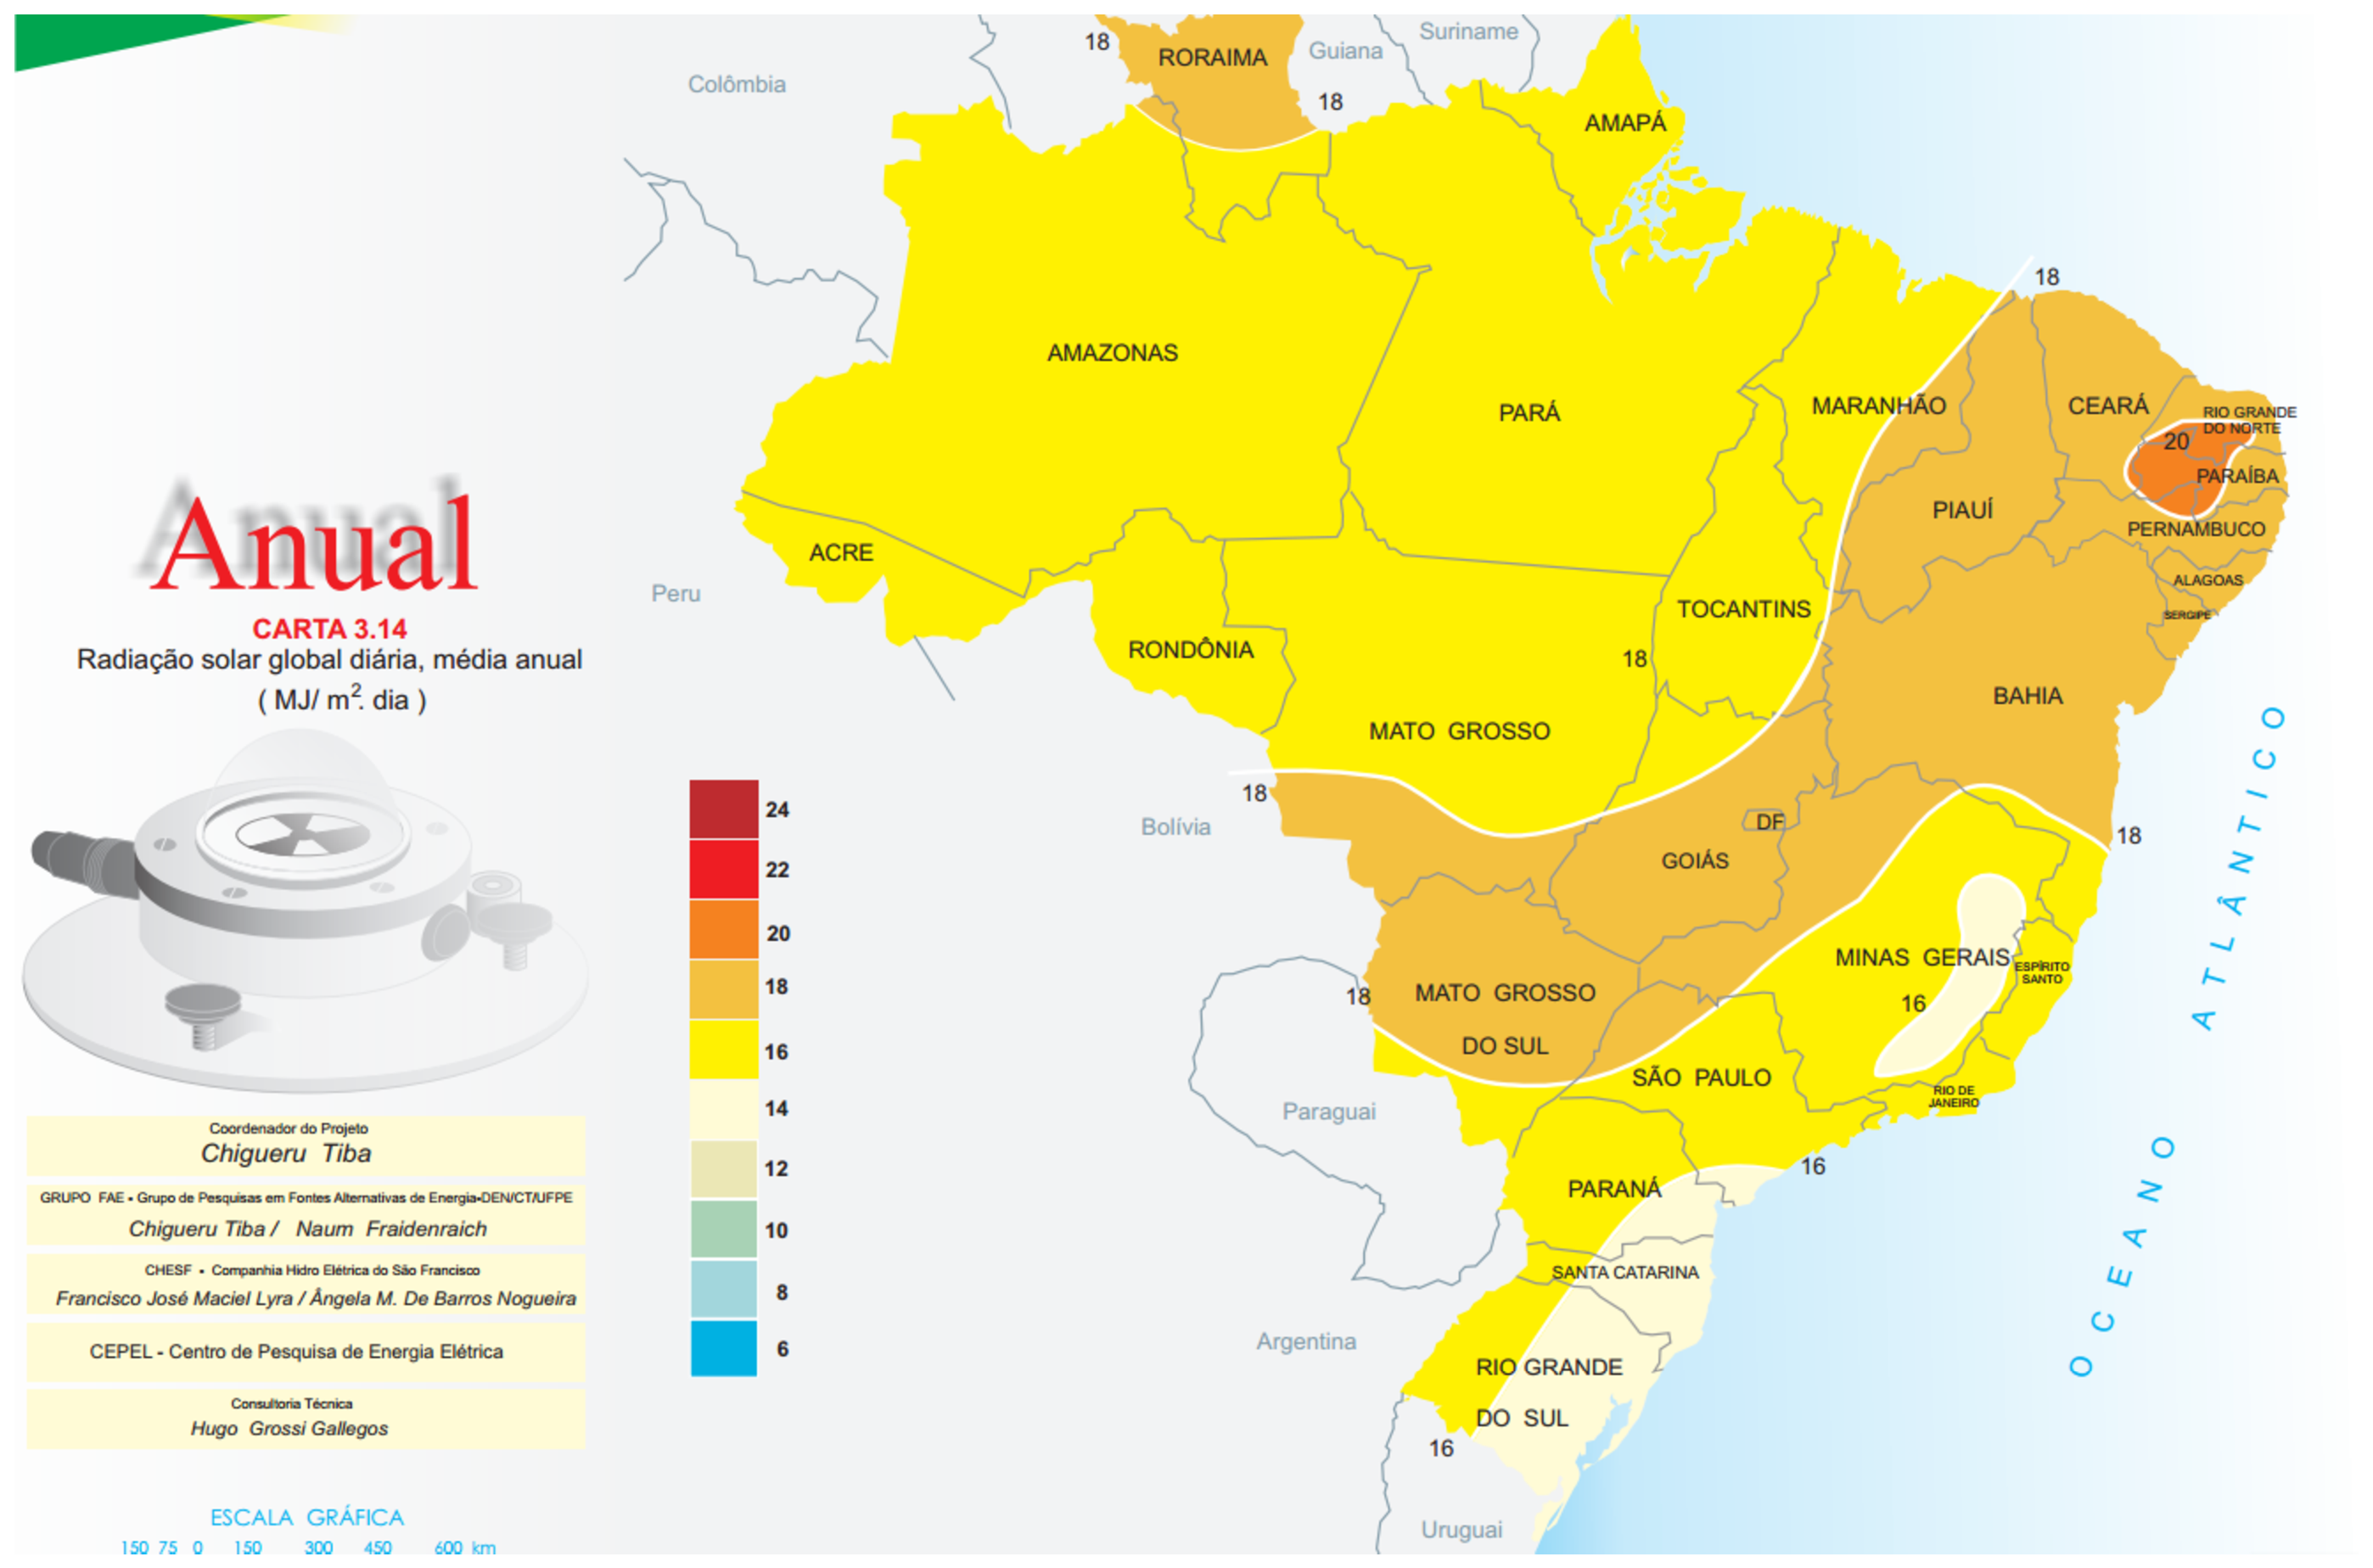
\includegraphics[width=.7\linewidth,keepaspectratio,angle=0]{figuras/radiacao_solar.eps}
\caption{Radiação solar global diária, média anual.}
\end{figure}

	A irradiação aproveitada pela fonte fotovoltaica é Irradiação Global Horizontal (GHI), onde quantifica em uma superfície plana a quantidade de radiação recebida. Esta radiação é divida em Irradiação Difusa Horizontal (DIF) e Irradiação Normal Direta (DNI). A DIF é uma quantidade dispersa por reflexões em elementos na atmosfera como poeira e as nuvens. A DNI é a irradiação que não sofre reflexões, atingindo o solo diretamente\cite{2012Energetica}.

	A determinação da posição dos painéis solares depende da variação da posição da Terra em relação ao Sol ao longo do ano, ao norte (azimute) e ao plano horizontal. Esta orientação otimiza aproveitamento solar de painéis fixos. Brasília está localizada no hemisfério Sul, logo os painéis deverão estar voltados para o norte “verdadeiro” e a inclinação de acordo com o plano horizontal. Esta inclinação pode ser de acordo com as estações do ano ou com a produção media durante o ano. A escolha deverá ser feita a fim de maximizar a produção\cite{2012Energetica}.

	Os elementos semicondutores fotossensíveis das placas fotovoltaicas fazem a conversão da  radiação solar em diferença de potencial nos terminais de junção P-N2, que é a junção metalúrgica de dois cristais de natureza P e N, de acordo com sua composição atômica. A corrente contínua é resultante da ligação elétrica desses terminais\cite{2012Energetica}.

	Segundo Fadigas\cite{14Fadigas}, a luz solar irá excitar a junção P-N e os fótons da luz irão se chocar com os elétrons da estrutura do silício. Desta forma, eles irão fornecer energia e transformara-os em condutores, criando um campo elétrico, no qual os elétrons fluem da camada P para a N, através de um condutor externo, gerando corrente elétrica (figura \ref{celula_fotovoltaica}).

\begin{figure}[H]
\centering
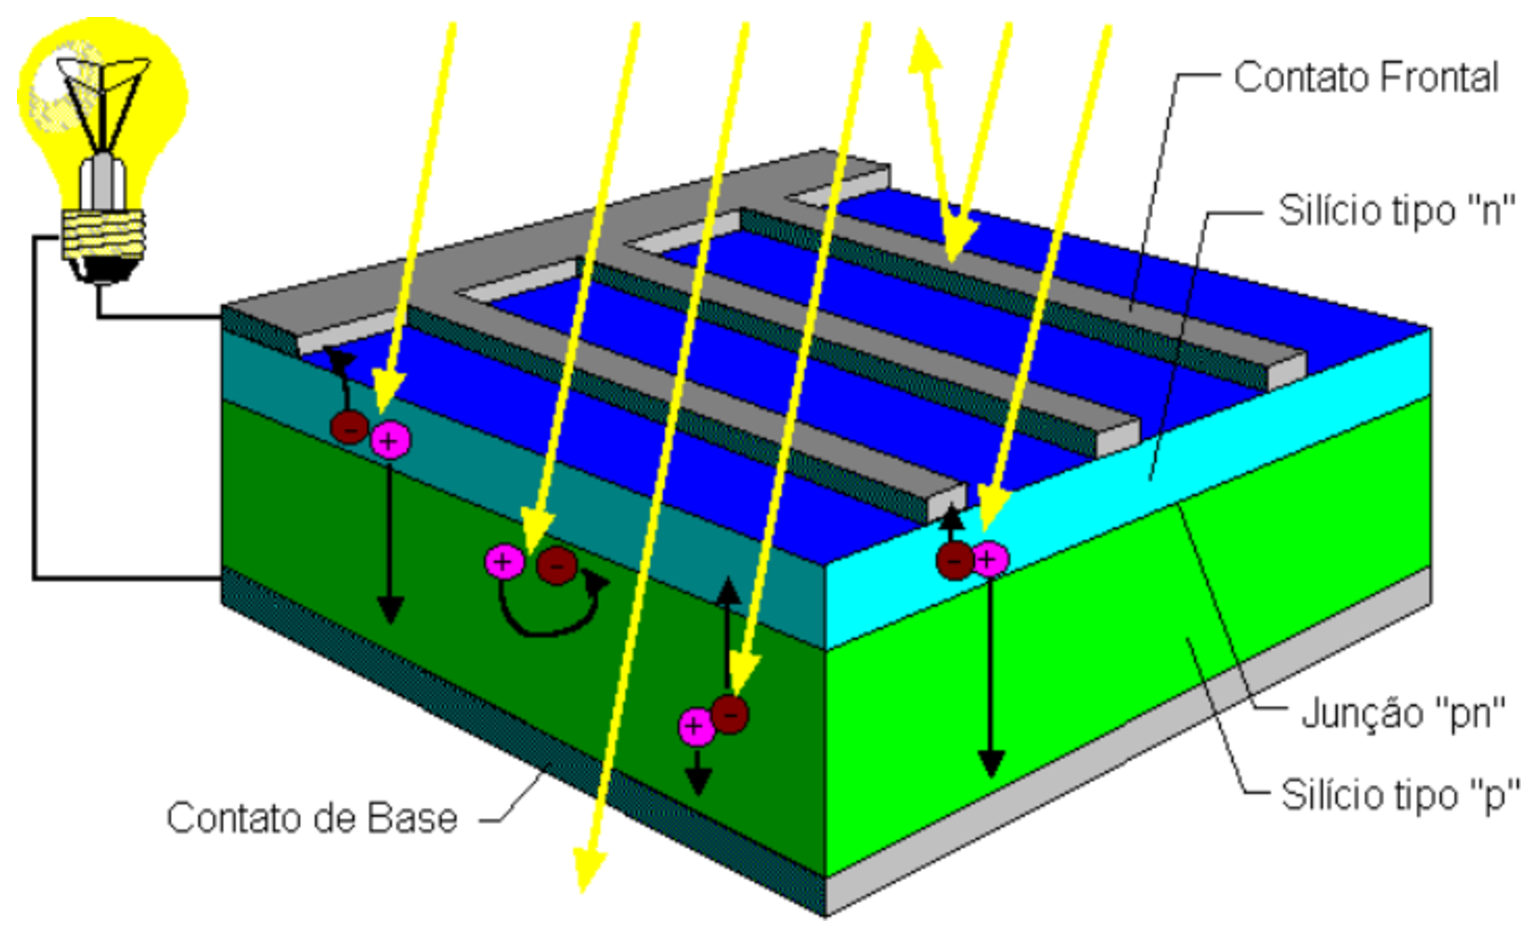
\includegraphics[width=.7\linewidth,keepaspectratio,angle=0]{figuras/celula_fotovoltaica.eps}
\caption{Célula fotovoltaica (corte transversal)\cite{1999CRESESBCEPEL}.}
\label{celula_fotovoltaica}
\end{figure}

	A condição de referência de eficiência do painel é a \textit{Standard Test Conditions} – STC, que estabelece a relação da potência máxima de saída pela área da célula em $\si{\meter}^{2}$ e o padrão é $1000\nicefrac{\si{\watt}}{\si{\meter}^{2}}$, a $25^{o}C$\cite{2012Energetica}.

	A temperature ambiente de operação e a intensidade da irradiação solar incidente sobre a célula são os principais fatores que interferem na eficiência da conversão. 

	De acordo com a Resolução Normativa 482/2012 da ANEEL, o sistema fotovoltaico da casa será uma minigeração distribuída pois a potência instalada será superior a 100 kW e inferior a 1 MW e estará conectada à rede de distribuição. O consumidor não poderá vender sua energia para a distribuidora, ela entrará no sistema de compensação de energia elétrica. A compensação de energia  funcionará da seguinte forma: o sistema de distribuição receberá a energia ativa da unidade consumidora e essa energia será cedida a título de empréstimo gratuito para a distribuidora. A unidade consumidora terá 36 meses para consumir esse crédito em quantidade de energia ativa\cite{42012ANEEL}.

\subsubsection{Eólica}

	O vento é o movimento horizontal e paralelo à superfície do planeta de parcelas de ar nas atmosferas planetárias. O vento é responsável pelo transporte de umidade e de energia na atmosfera como agente meteorológico. Já sua energia provoca grande destruição como furações e tornados. Porém, ele pode ser aplicado como uma fonte alternativa de energia, transformando energia cinética em eletricidade\cite{52008Martins}.

	A energia cinética que está contida no vento é convertida em energia mecânica pelo giro das pás do rotor das turbinas eólicas. E depois é transformada em energia elétrica pelo gerador. A potência $p$ do vento e a velocidade u através de uma área A (área das hélices que interceptam o vento) é dada por:

$p\ =\ \cfrac{1}{2}\rho A u^{3}$

	No qual $\rho$ é a densidade do ar. A máxima potência de uma turbina eólica é 59\%, mas ao  somar as perdas mecânicas, a potência total do vento utilizável reduz para 42\%\cite{52008Martins}.

	O potencial eólico brasileiro também consideravelmente grande em comparação com vários outros países. Como pode ser visto na figura \ref{potencial_eolico}, o Brasil é capaz de produzir $272,2 \si{\tera\watt\hour}$ por ano. Contudo, o potencial da região Centro-Oeste é o menor dentre as 5 regiões brasileiras, com $5,4\si{\tera\watt\hour}$ por ano. O segundo menor que é a região Norte tem a capacidade produzir $26,4\si{\tera\watt\hour}$ por ano. 

\begin{figure}[H]
\centering
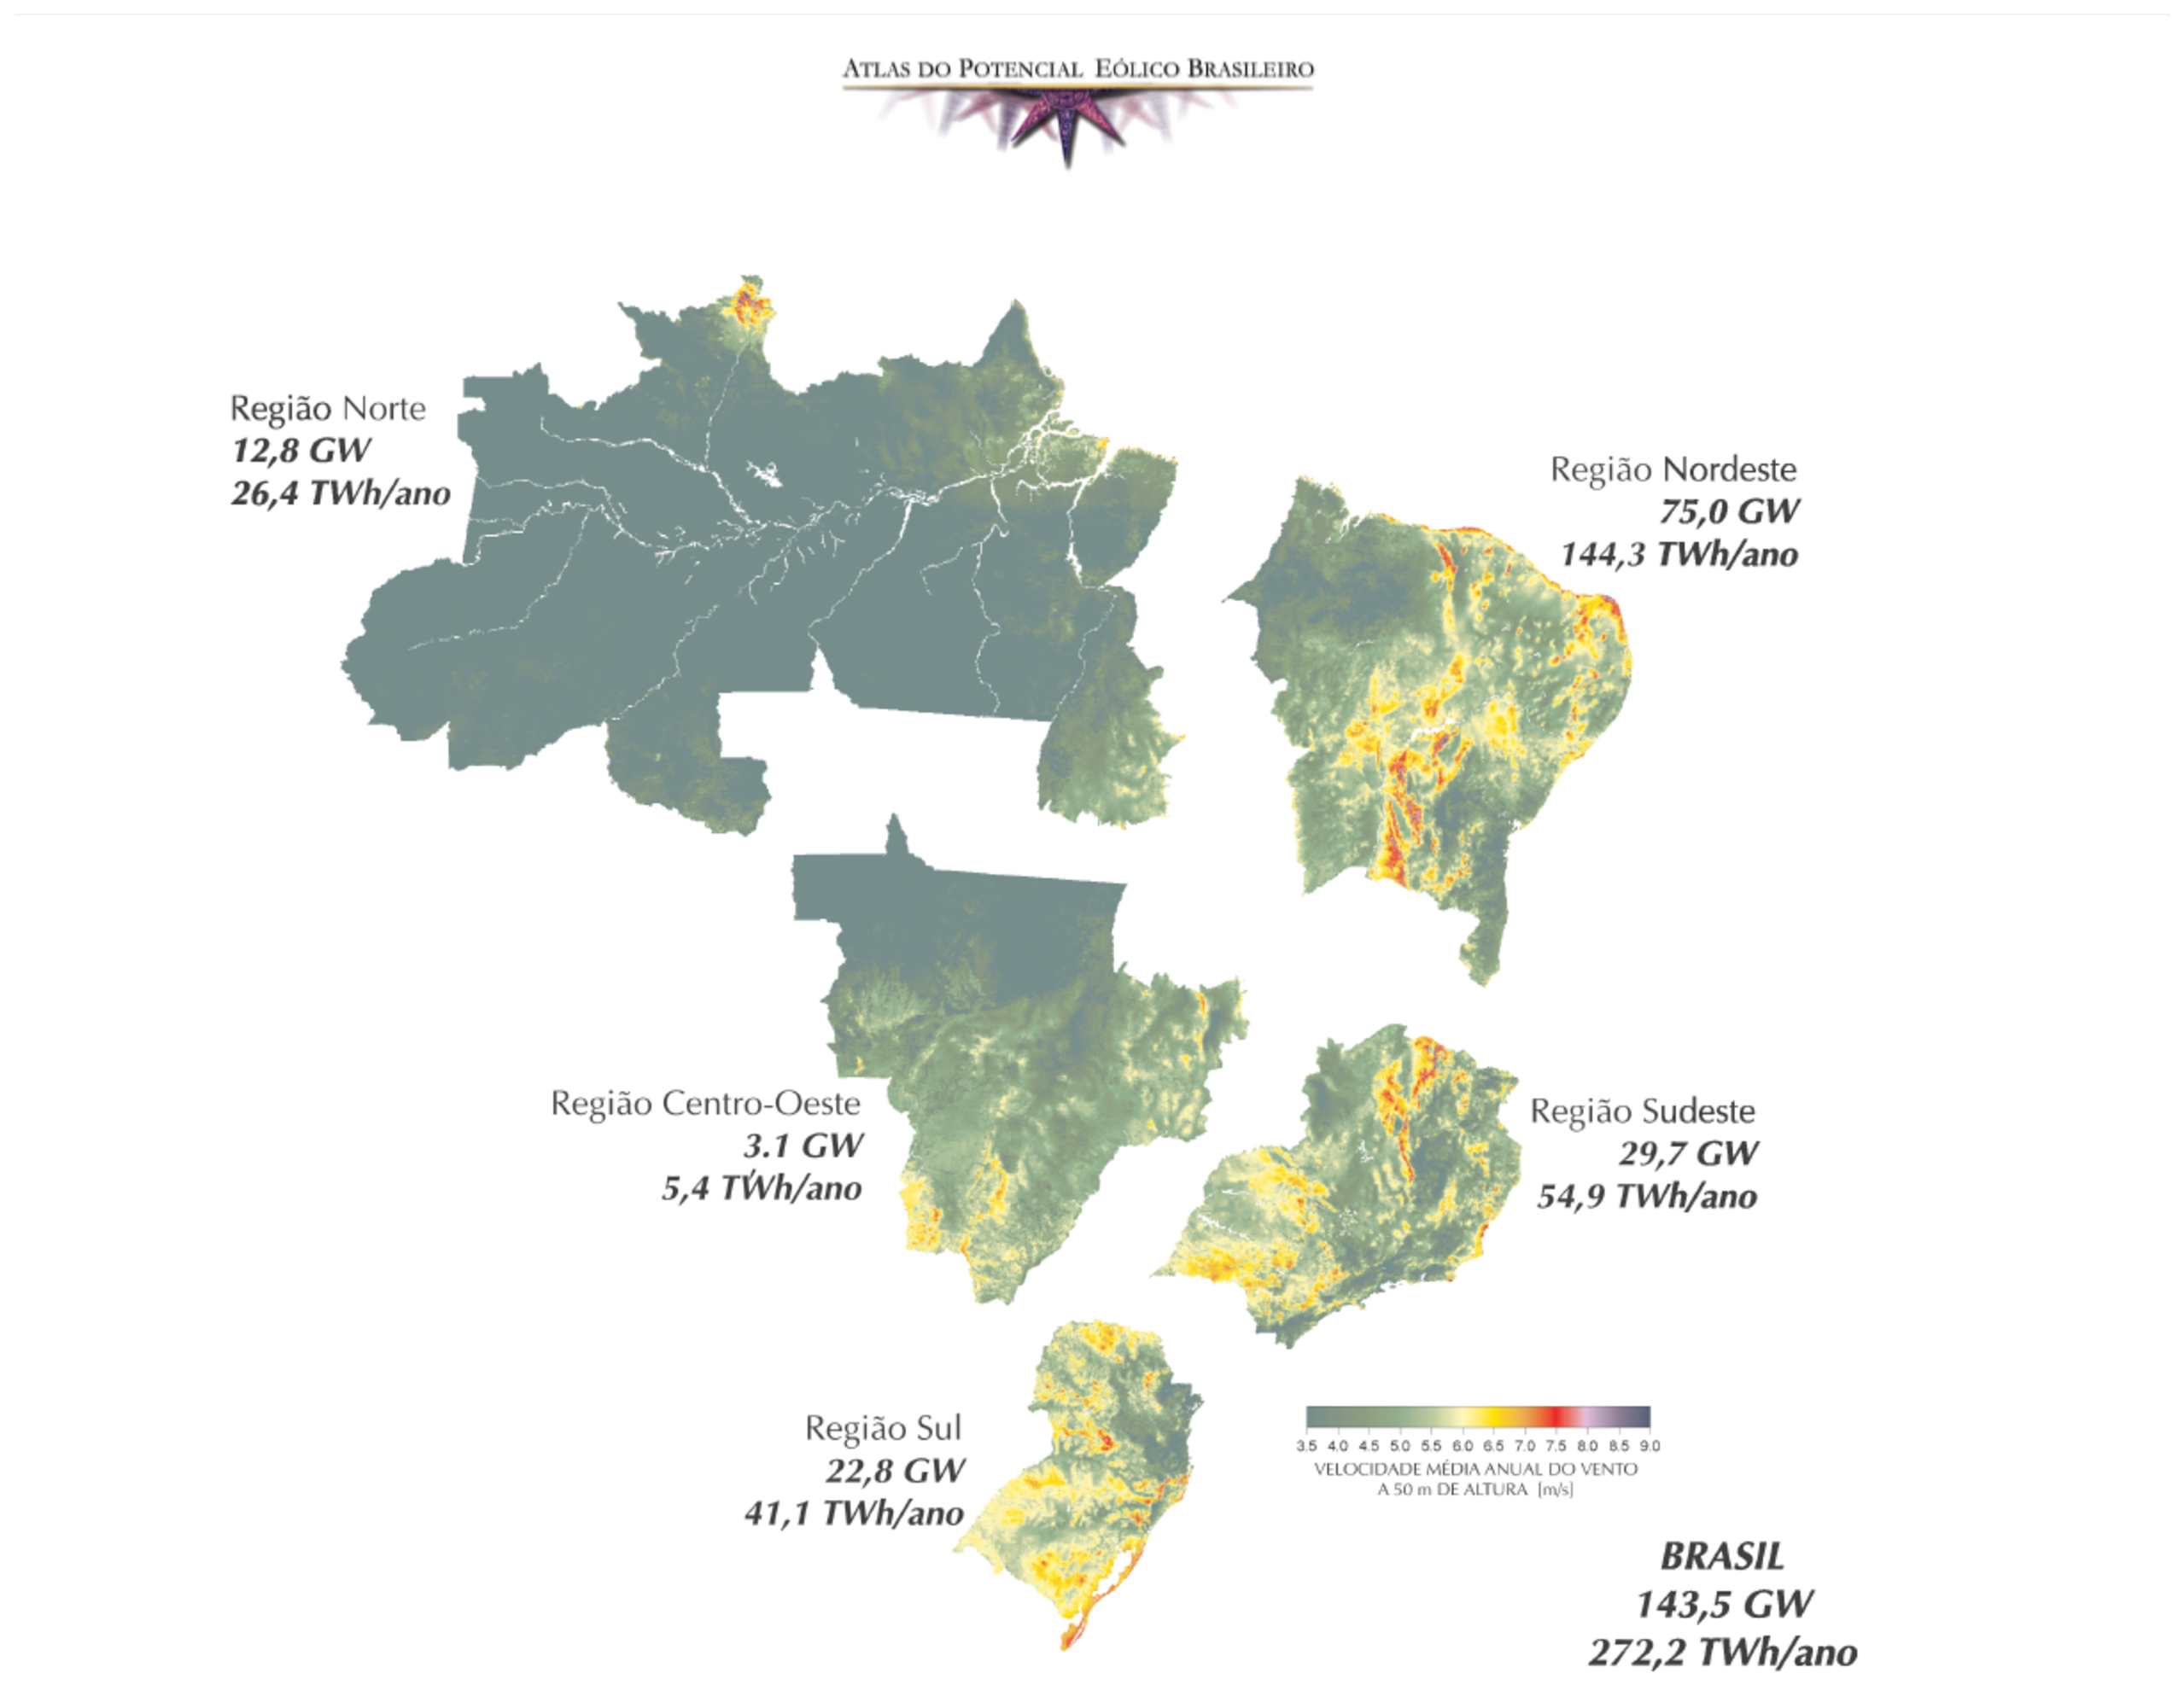
\includegraphics[width=.7\linewidth,keepaspectratio,angle=0]{figuras/potencial_eolico.eps}
\caption{Potencial eólico para vento médio anual igual ou superior a $7\nicefrac{\si{\meter}}{\si{\second}}$\parnote.}
\label{potencial_eolico}
\end{figure}

	A velocidade média anual do vento no Distrito Federal é 3,5m/s (Figura 4). Essa velocidade é suficiente para produzir uma pequena quantidade de energia. A fim de aproveitar essa energia e de solucionar outro problema, a energia eólica também será utilizada no projeto da casa. De acordo com Cormane (2015, por questão de segurança, quando houver falta de energia elétrica por parte da distribuidora, o sistema da casa também deverá ser desligado. Isso deverá ocorrer porque, caso haja necessidade de reparo da rede de alta tensão, não poderá haver energia passando pela rede porque operários poderão estar trabalhando nela o que causará um acidente fatal. 

	Desta forma, a energia eólica será responsável por abastecer um banco de baterias. Estas ficariam responsáveis por abastecer a casa em casos de falta de energia. Para que esse processo ocorra, será necessário fazer um sistema em que no momento que a energia elétrica acabasse, a casa ficaria ilhada da rede. Em outras palavras, a casa funcionaria em dois sistemas, grid-tie e off-grid, mas não ao mesmo tempo. Grid-tie quando houvesse energia na rede de distribuição e off-grid quando acabasse. A casa ficaria isolada do sistema, e as baterias iriam alimentar os principais pontos e eletrodomésticos da casa como geladeira e sistema de segurança.

\begin{figure}[H]
\centering
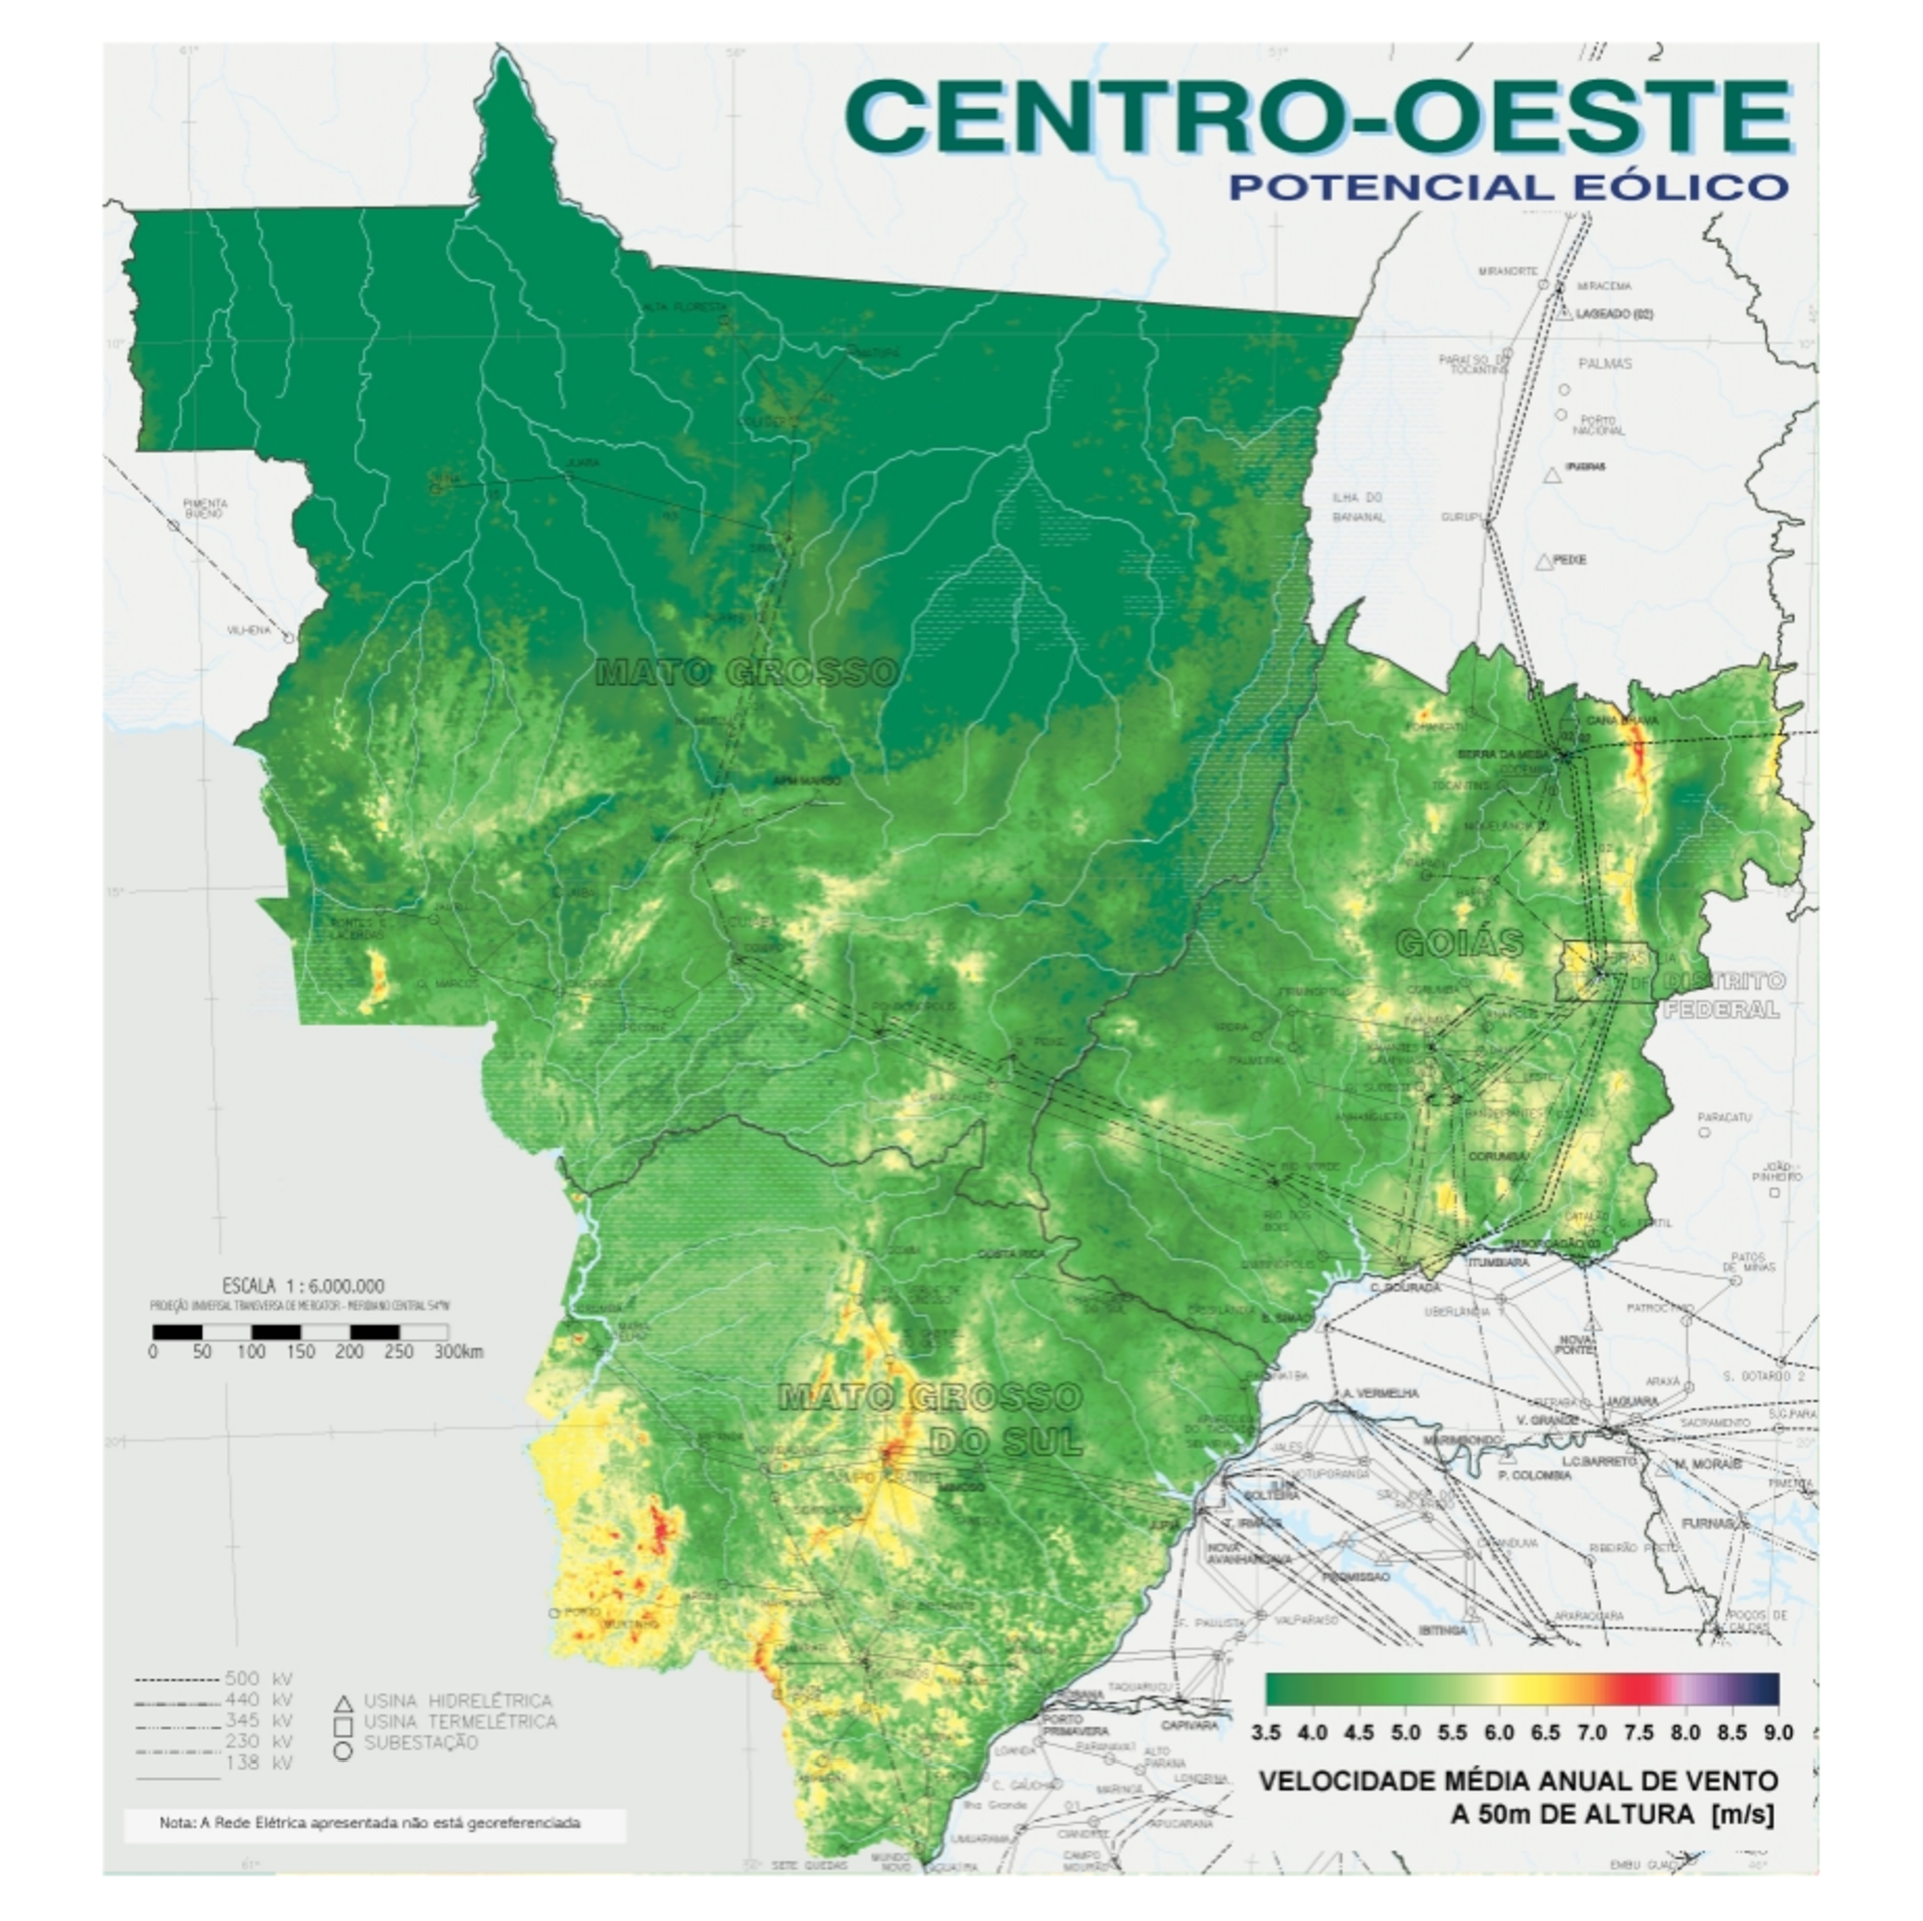
\includegraphics[width=.65\linewidth,keepaspectratio,angle=0]{figuras/potencial_centro_oeste.eps}
\caption{Potencial eólico na região Centro-Oeste.}
\label{potencial_centro_oeste}
\end{figure}

\begin{table}[H]
\centering
\begin{tabular}{|c|c|c|c|c|}
\hline 
\multirow{2}{*}{\textbf{Fontes}} & \textbf{Custo de implantação} & \multirow{2}{*}{\textbf{Eficiência}} & \textbf{Emissão de poluentes} & \multirow{2}{*}{\textbf{Manutenção}}\tabularnewline
 & \textbf{CESP/IMT {[}U\$/W{]}} &  & \textbf{{[}gCO2/kWh{]}} & \tabularnewline
\hline 
\hline 
Eólica & 1,00 & 42\% & 9,5 & Baixo custo\tabularnewline
\hline 
Solar & 5 à 10 & 15,4\% & 32 & Baixo custo\tabularnewline
\hline 
\end{tabular}
\caption{Comparativo entre solar e eólica}
\label{comparativo_solar_eolica}
\end{table}

A tabela \ref{comparativo_solar_eolica} mostra uma comparação entre as duas fontes que serão usadas no projeto da casa sustentável. A energia solar, a princípio, será mais cara, mas com o tempo o seu custo será pago. E depois o consumidor irá receber lucros com a sua implantação. A energia eólica já está com um preço de mercado para concorrer com as outras fontes. Desta forma, a utilização destas fontes é vantajosa para o empreendimento pois o consumidor não terá prejuízo com sua implantação.

\subsection{Dimensionamento}

	Para o dimensionamento e justificativa das fontes de energia, atribuiu-se que o consumo da residência seja de 500\nicefrac{\si{\kilo\watt\hour}}{mês} por motivos de segurança, já que o valor estimado na Tabela referente ao consumo mensal dos eletrodomésticos.

\subsection{Conexão dos painéis solares}

	As placas fotovoltaicas serão on-grid, ou seja, conectadas à rede elétrica da concessionária. O consumo mensal estipulado é de 500\si{\kilo\watt\hour} por mês. Logo, se trata de um sistema trifásico. Para que o sistema on-grid seja efetuado, é necessário a adesão obrigatória de uma taxa de disponibilidade da companhia energética, no qual de 100\si{\kilo\watt\hour} por mês. Portanto, o sistema será dimensionado para 400\si{\kilo\watt\hour} mensal [ANEEL -  Resolução Normativa ANEEL n$^o$ 482/2012].

\subsection{Stringbox}
	
	Caixas de string ou string box são caixas elétricas que estão conectadas nas placas solares, inversor e no quadro geral da casa. Sua função é de defender o sistema em caso curtos, sobrecargas e surtos nele estão localizados fusíveis, disjuntores e DPS.

	O Fusível está alocado no sistema com a finalidade de proteger o sistema de curtos-circuitos, caso a intensidade da corrente elétrica supere o valor determinado, o fusível se rompe e corta o fornecimento, evitando assim que haja danificação em aparelhos importantes. Hoje em dia a maioria dos inversores residenciais já possui dentro de si fusíveis, tornando dispensável a alocação desse componente de proteção na string box.

	O Disjuntores nada mais é que um interruptor automático que é destinado a proteger o inversor e o sistema elétrico da casa, em cada string box haverá dois disjuntores. Sua função nada mais é detectar picos de corrente que ultrapassem o necessário para o circuito interrompendo-a antes que os seus efeitos possam causar danos à instalação.
	
\textbf{Dispositivo de Proteção contra Surtos Atmosféricos} (DPS) se assemelha ao Para raios, porém é instalado em paralelo ao disjuntor no quadro da string box. O DPS protege diretamente a rede elétrica interna e o Inversor de um surto atmosférico externo, conduzindo através da rede a descarrega para a terra.

Abaixo pode-se ver o diagrama do funcionamento de uma string box, a energia gerada por painéis fotovoltaicos é levada até o primeiro disjuntor, é valido lembrar que a energia gerada por essas placas é de corrente continua, então cria-se uma necessidade de se usar um disjuntor de corrente continua, em paralelo a ele será alocado um DPS de corrente continua, para evitar distúrbios vindos de raios. Logo em seguida está aloca-se o Inversor Grid-tie que estará em série ao disjuntor, ele tem a função de transformar a corrente continua em corrente alternada, no inversor também está alocado os fusíveis dando assim mais segurança ao sistema. Após a conversão os cabos são alocados novamente na string box, porém em um disjuntor para corrente alternada em paralelo a ele há mais um DPS também de corrente alternada, para evitar que surtos vindos da rede não queimem nenhum dos componentes de geração da Green House.

	No Mercado há uma infinidade de opções para a montagem de uma string box, desde quadros prontos até a compra de componente por componente. Após uma pesquisa em sites de venda de acessórios para geração de energia solar observou-se que o preço médio de umastring box pronta é entorno de 1500 reais, mas caso seja escolhida a opção de comprar componente por componente esse preço cai pela metade, já que é possível comprar materiais de marcas diferentes e qualidades diferentes, é valido informar que o funcionário deve ter um conhecimento breve sobre string box, antes de fazer a construção de uma.

\begin{figure}[H]
\centering
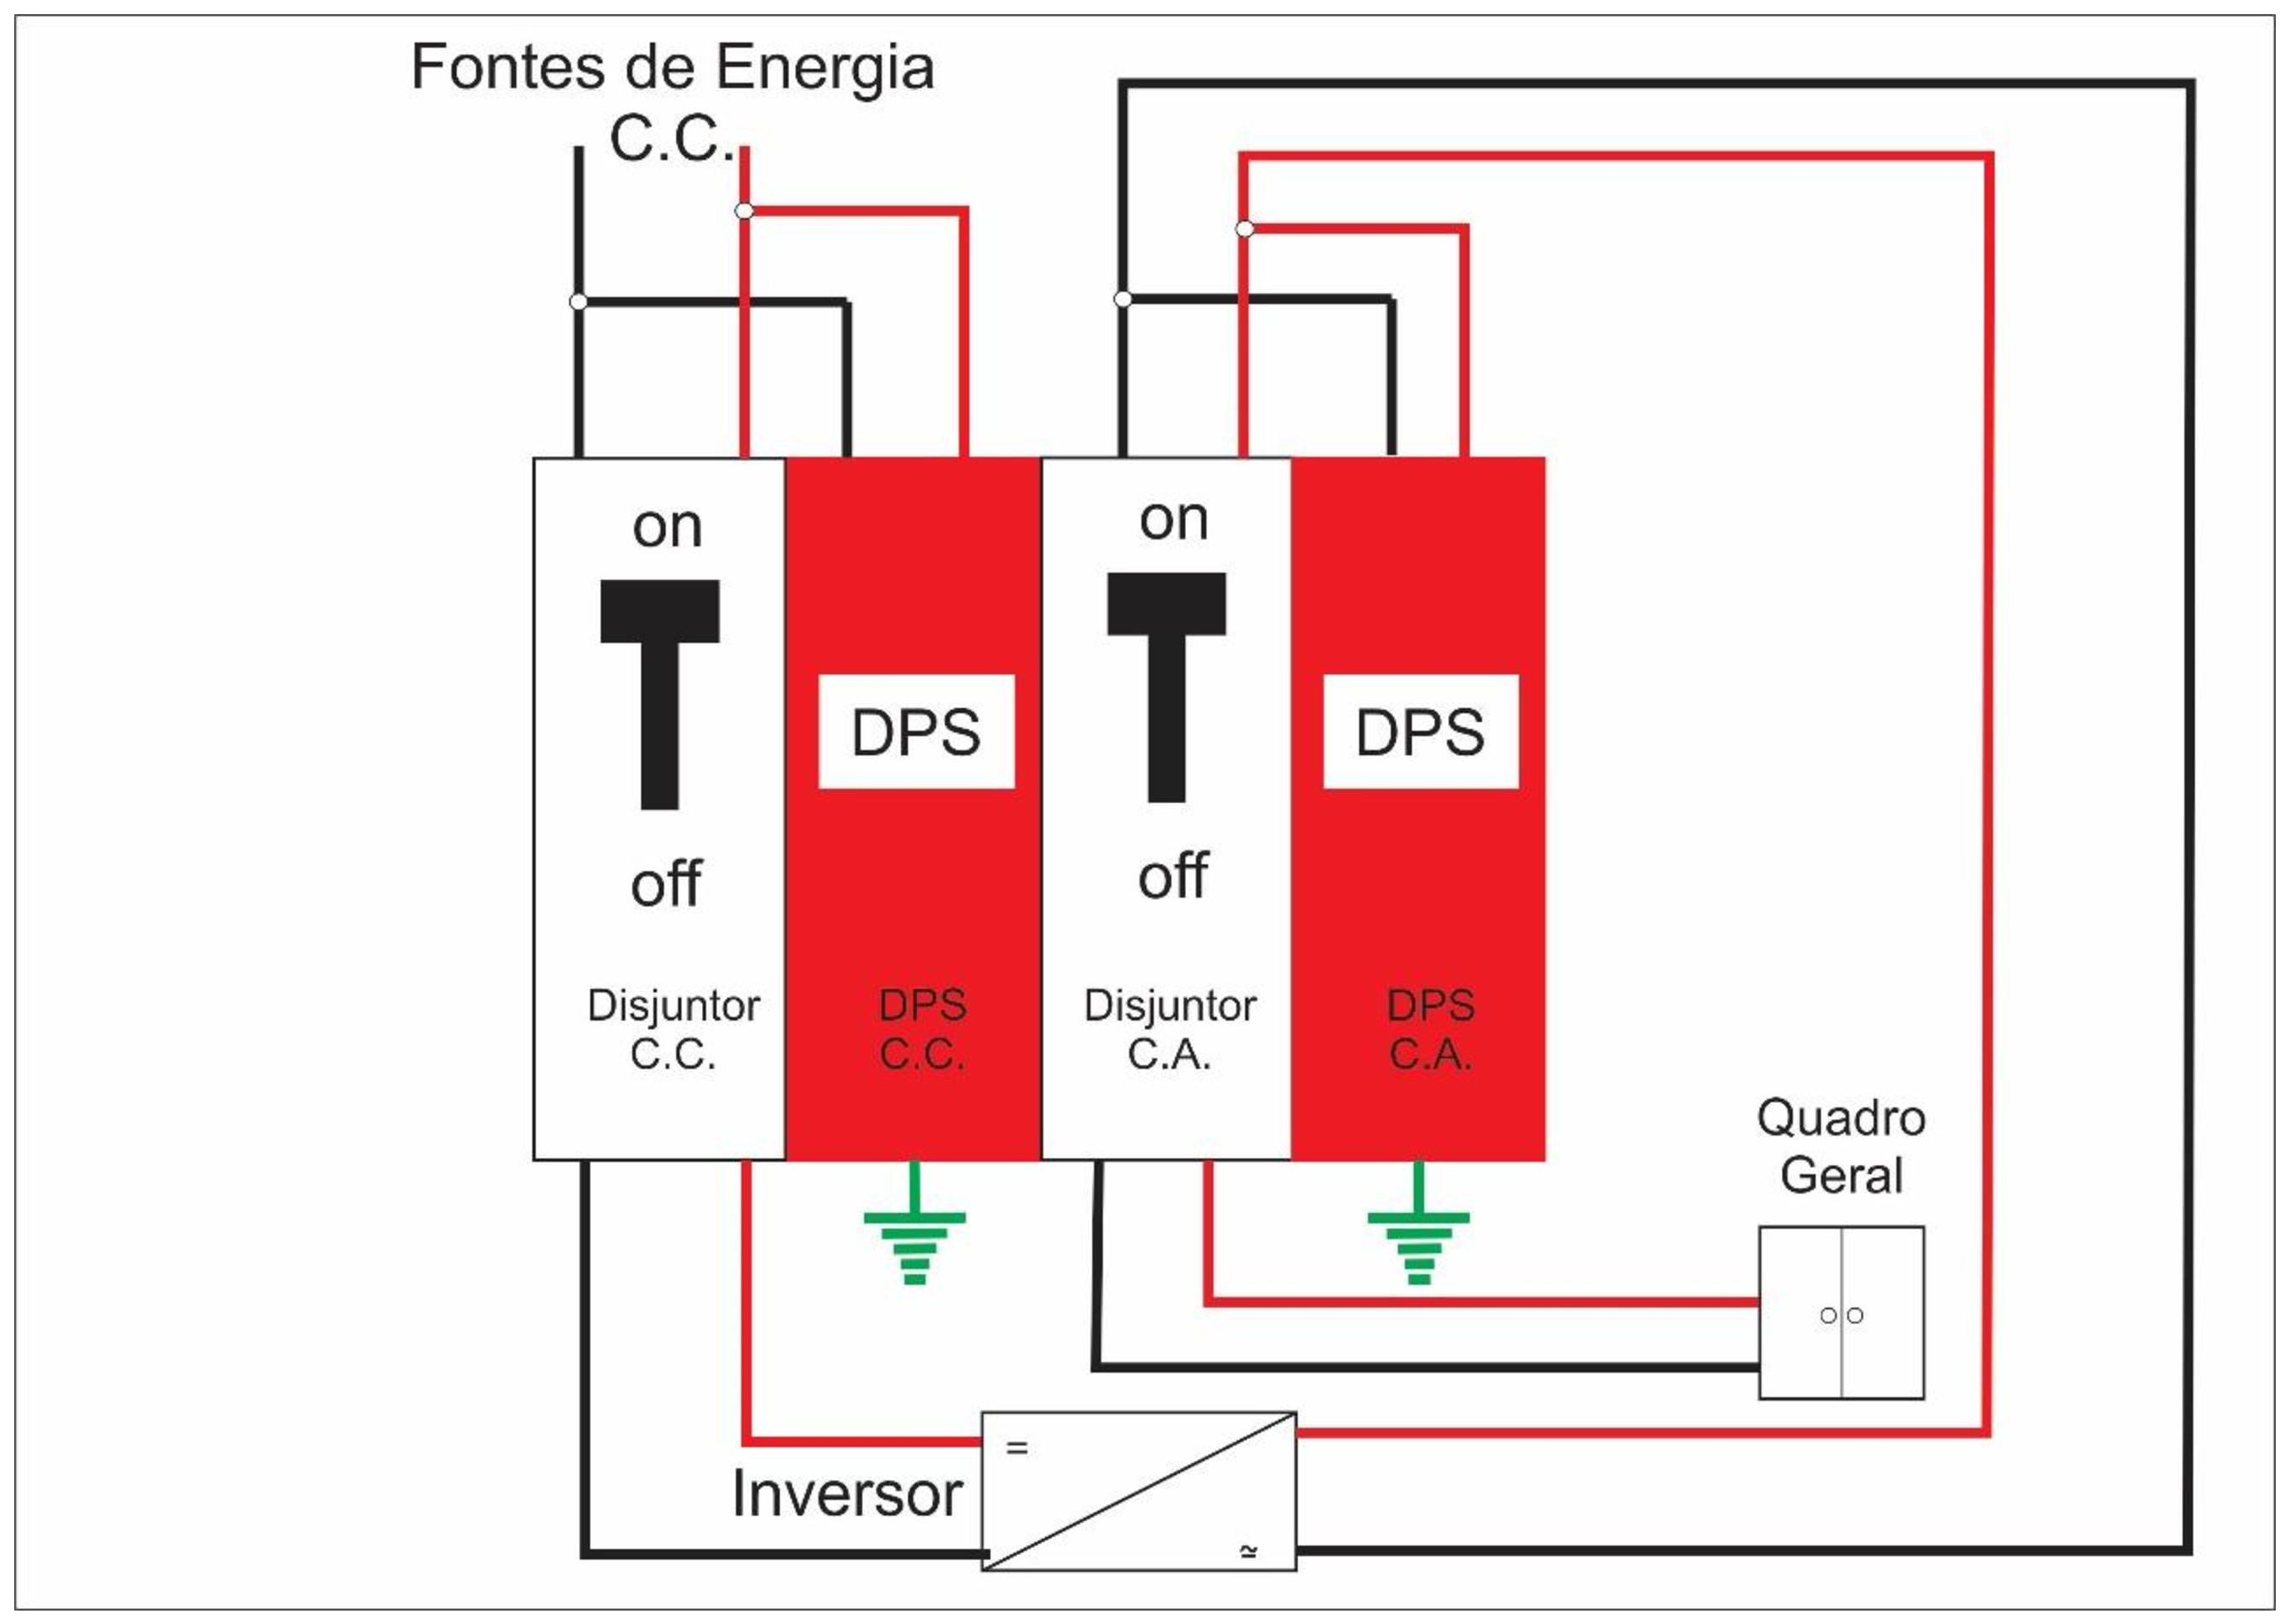
\includegraphics[width=.75\linewidth,keepaspectratio,angle=0]{figuras/stringbox_esquematico.eps}
\caption{Esquemático de montagem da Stringbox.}
\label{stringbox_esquematico}
\end{figure}


\subsection{Quantidade de placas solares}

	Para determinar o número de placas solares, primeiro necessita-se conhecer a quantidade de energia consumida diariamente. Para isso basta fazer um cálculo simples onde se divide a energia mensal pelo número de dias. Sendo: energia consumida = 400 \nicefrac{\si{\kilo\watt\hour}}{mês} = 13,33 \nicefrac{\si{\kilo\watt\hour}}{dia}. Em seguida, precisa-se conhecer o índice solarimétrico médio por dia em Brasília \cite{ufpe2000}. Esse índice determina a quantidade de irradiação solar o local recebe por dia.

	Índice solarimétrico local de Brasília: $I_s = 5,13 \nicefrac{\si{\hour}}{dia}$

	Por fim, a potência das placas é definida a partir da razão entre a energia consumida pelo índice solarimétrico:

	$P_p\ =\ \dfrac{13333,33}{I_s}\ =\ 2600 \si{\watt}$

	Considerando uma eficiência de 0,85\%, devido a perdas de geração e transmissão,

	$P_t\ =\ \dfrac{2600}{0,85}\ =\ 3060 \si{\watt}$

	Com a placa de potência de 255 W, pode-se obter a quantidade de painéis solares a partir da seguinte expressão:

	$N_{placas}\ =\ \dfrac{3060}{255}\ =\ 12$ placas no total

	Logo, serão necessárias \textbf{12 placas de 255 \si{\watt}}.


\subsection{Direção de instalação das placas para melhor geração de energia}

	A melhor direção para a instalação dos painéis é virada para a linha do Equador, no caso de Brasília está voltada para a direção Norte. Contudo, se houver um elevado nível de sombreamento nesta direção, sugere-se que os painéis então sejam colocados na face leste ou oeste do telhado da residência. Sabendo que, essa escolha poderá influenciar na quantidade de energia gerada. Vale enfatizar que, essas especificações visam a grosso modo o melhor aproveitamento da incidência solar na hora de instalar os módulos, pois há outras condições e variáveis que devem ser analisadas com mais cautela. 

	No que se diz respeito à inclinação dos painéis, é importante que eles estejam a maior parte do período de insolação perpendiculares à direção de radiação solar, ou seja, igual ou o quão próximo possível à latitude da região. No caso, a melhor angulação para as placas deverá ser igual à 15,4\si{\degree}.

\subsection{Especificações do aerogerador}

	A média, de acordo com o Atlas Eólico Brasileiro, de Brasília é 3,5 \nicefrac{\si{\meter}}{\si{\second}}. Logo, a potência gerada por essa velocidade será baixa. A energia produzida pelo vento será destinada para abastecimento das baterias de reserva, que funcionarão caso acabe a energia devolvida pela concessionária da rede elétrica.

	No mercado mundial de aerogeradores são produzidos diversos modelos e com diferentes especificações técnicas que se adaptam melhor às necessidades de cada um. Os modelos são separados em duas categorias, sendo eles: aerogerador de eixo horizontal e de eixo vertical. Como a energia eólica será uma fonte secundária, escolheu-se dois exemplares (um de cada modelo) de potência baixa.

\begin{table}[H]
\begin{tabular}{|c|c|c|}
\cline{2-3}
\multicolumn{1}{c|}{} & \multicolumn{2}{c|}{\textbf{Aerogerador}}\tabularnewline
\cline{2-3}
\multicolumn{1}{c|}{} & \textbf{Eixo Vertical}\parnote{Aeolos Wind Turbine 600[\si{\watt}]} & \textbf{Eixo Horizontal\parnote{Air 40}}\tabularnewline
\hline
Energia & 100kWh/mês - 5,8 m/s & 40kWh/mês - 5,8 m/s\tabularnewline
\hline
Velocidade de arranque & 1,5 m/s & 3,1 m/s\tabularnewline
\hline
Faixa de velocidade  & \multirow{2}{*}{1,5 - 40 m/s} & \multirow{2}{*}{3,1 - 22 m/s}\tabularnewline
de geração  &  & \tabularnewline
\hline
Ruído & < 45 dB & Silencioso\tabularnewline
\hline
Altura da torre & 1,6 metros & 10 metros\tabularnewline
\hline
Garantia & 5 anos & 5 anos\tabularnewline
\hline
Manutenção & Livre & Livre\tabularnewline
\hline
Vida útil & 20 anos & 20+ anos\tabularnewline
\hline
Local da compra & Reino Unido & Brasil\tabularnewline
\hline
Preço & R\$ 3.600,00 \parnote{Preço diretamente convertido em reais com a cotação do dolar à R\$ 4,07 referente ao dia 01/11/2015}$\ $ \parnote{Valor em tólar U\$ 849,00} & R\$ 5.499,00\tabularnewline
\hline
\end{tabular}
\parnotes
\caption{Quadro comparativo entre os modelos de aerogeradores}
\label{aerogeradores_modelos}
\end{table}

A escolha do aerogerador de eixo horizontal se deve ao fato deste estar mais presente no mercado, com mais opções. Além do mais, a garantia é brasileira. Já o aerogerador de eixo vertical seria importado, aumentando os custos devido à alta do dólar e os impostos.

	O aerogerador a ser utilizado é o \textbf{Air 40}.


\subsection{Localização e altura de instalação do aerogerador para otimização do potencial eólico}

	Quanto mais alto e direcionado para uma longa região livre de obstáculos aéreos, melhor. Pela sugestão do fabricante, e informações fornecidas pelo Profº Drº Jorge Cormane Universidade de Brasília/FGA, a melhor eficiência estará no aerogerador instalado acima de 10 metros do chão. Por ser pequeno, quando comparado aos aerogeradores de grande geração, o Air 40 pode ser instalado no teto da casa, com o suporte de uma haste para prolongar sua altura referente ao solo.

\subsection{Períodos de manutenção}

	O período de manutenção dos painéis não necessita de ser feita com uma determinada periodicidade, porém é preciso estar sempre atento aos sistemas de monitoramento e controle da energia produzida pelos painéis, sendo necessária a vistoria e limpeza em caso de queda na quantidade da potência.

	Já a limpeza dos módulos fotovoltaicos deve ser realizada na parte frontal, para que a eficiência não seja interferida, com o uso de um pano de microfibras e etanol sobre o vidro. Sendo esta realizada num período de 6 meses.

\subsection{Quadro comparativo entre os modelos de placas solares}

	De acordo com o material escolhido para a placa, silício cristalino, devido às suas propriedades e melhor eficiência dentre os painéis de outros materiais. Comparou-se duas placas de 255\si{\watt} de silício monocristalino. As duas placas possuem garantia de 25 anos (80\% de eficiência).

\begin{table}[H]
\centering
\begin{tabular}{|c|c|c|c|c|c|c|}
\hline 
\textbf{Modelo} & \textbf{Vida útil} & \textbf{Máx.} \si{\volt} & \textbf{Temp.}\si{\celsius} & \textbf{Peso} [\si{\kilo\gram}] & \textbf{Dimensão} [\si{\milli\meter}] & \textbf{Preço} R\$\tabularnewline
\hline 
\hline 
ISOFOTON & \multirow{2}{*}{30 anos} & \multirow{2}{*}{1000\si{\volt}} & \multirow{2}{*}{$-40\si{\celsius}$ até $+85\si{\celsius}$} & \multirow{2}{*}{19} & \multirow{2}{*}{$1667\times994\times45$} & \multirow{2}{*}{1.453,15}\tabularnewline
ISF-255 &  &  &  &  &  & \tabularnewline
\hline 
MITSUBISH & \multirow{2}{*}{35 anos} & \multirow{2}{*}{600\si{\volt}} & \multirow{2}{*}{-} & \multirow{2}{*}{20} & \multirow{2}{*}{$1625\times1019\times46$} & \multirow{2}{*}{1.400,00}\tabularnewline
I 255 &  &  &  &  &  & \tabularnewline
\hline 
\end{tabular}\caption{Comparação entre as placas fotovoltaicas}
\label{comparacao_fotovoltaicas}
\end{table}

Comparando as duas placas acimas, a que melhor se encaixa no perfil do projeto da casa é a MITSUBISHI 255W porque é possui uma vida útil maior, é mais barata e a garantia é oferecida dentro do Brasil. Ao contrário da placa ISOFOTON ISF-255 que não possui garantia dentro do
Brasil e o seu valor final dependerá da flutuação do dólar.

\subsection{Valor dos painéis utilizados}
	O projeto irá utilizar 12 painéis de 255W. Como foi escolhido o painel acima. O valor total dos painéis será:

	$$V_T\ =\ 12\times1.400,00 = 16.800,00$$

	Logo, o valor total será R\$16.800,00.

%%%%%%%%%%%%%%%%%%%%%%%%%%%%%%%%%%%%%%%%%%%%%%%%%%%%%%%%%%%%%%%%%%%%%%%%%%%%%%
%%%%%%%%%%%%%%%%%%%%%%%% Tecnologia de Armazenamento %%%%%%%%%%%%%%%%%%%%%%%%%
%%%%%%%%%%%%%%%%%%%%%%%%%%%%%%%%%%%%%%%%%%%%%%%%%%%%%%%%%%%%%%%%%%%%%%%%%%%%%%

\section{Tecnologia de Armazenamento}

\subsection{Definição de tecnologia de armazenamento}

	As tecnologias de armazenamento tem como intuito “guardar” a energia gerada pelos painéis solares e o aerogerador e transformá-la em eletricidade, e o excedente ser depositado em algum “lugar” ou alocado. Podendo ser elas em forma de baterias, acumuladores de energia, ou sistemas inteligentes interligados à rede elétrica.

\subsection{Tecnologias Utilizadas}

	Para o armazenamento das energias geradas pelos painéis solares e pelo aerogerador, têm-se duas propostas, sendo uma o uso de baterias residenciais e a outra consiste num sistema grid-tie em que serve para "jogar" na rede elétrica a energia excedente. Como o sistema grid-tie funciona apenas para fazer uma espécie de troca de energia com a companhia de energia elétrica, isso não impede que a casa sofra quedas de energias e apagões. Por ser a fonte primária de geração de energia e mais eficientes, os painéis solares serão ligados ao sistema com a rede. Já a energia produzida pelo aerogerador servirá para recarregar e armazenar em baterias. O uso das baterias tem como premissa a continuidade do fornecimento de eletricidade na casa, mesmo em apagões.

	As tecnologias de armazenamento mais comuns e que se adequam às necessidades da casa são: o uso de baterias residenciais e um sistema grid tie.

\subsection{Funcionamento}

	Sistemas Grid-Tie, se refere a um dispositivo eletrônico que permite aos usuários de energia solar ou eólica interligar seus sistemas com a rede da concessionária e injetar na rede o excedente de energia produzido pelos sistemas (fotovoltaico ou eólico). Esse sistema gerará um custo inicial alto, porém a sua manutenção é demorada e o retorno quanto a economia e o custo da energia elétrica oferecida pelas concessionárias compensa em pouco tempo de uso.

	Se trata de um dispositivo eletrônico que será conectado aos painéis solares, interligando seus sistemas com a rede da concessionária e injetando na rede o excedente de energia produzido. Funcionando da seguinte forma, quando proprietário do sistema produzir mais energia do que consome, a energia produzida fará com que o medidor “gire para trás”. Quando produzir menos do que consome, o medidor deverá “girar mais devagar”. Vale observar que o medidor deve ser apropriado para contabilizar o fluxo de energia nos dois sentidos.

	Já as baterias residenciais servirão para armazenar parte da energia produzida e utilizadas quando houver picos de energia quanto à energia retornada pela concessionária, ou afim de economia referente às tarifas. Atualmente, têm-se as baterias automotivas que são mais encontradas para fazer esse tipo de armazenamento, porém para isso deve-se fazer algumas adaptações e associar um grande número de baterias para que elas consigam reabastecer de forma significante a eletricidade da casa. Em contrapartida, recentemente a empresa especializada em automóveis elétricos \cite{TESLA} apresentou no início do ano (2015) baterias feitas para o uso residencial, a PowerWall. Tais baterias tem como proposta melhorar a autonomia da casa em relação à dependência da companhia energética local. Com duas capacidades, a \cite{TESLA} apresenta o modelo de bateria residencial com capacidade de armazenamento de 7kWh e 10kWh, custando respectivamente U\$ 3000 e U\$ 3500. Já disponíveis para compra no site da empresa. As baterias podem ser associadas em série e afixadas a qualquer lugar da casa \cite{TESLA}.

\begin{figure}[H]
  \begin{center}
	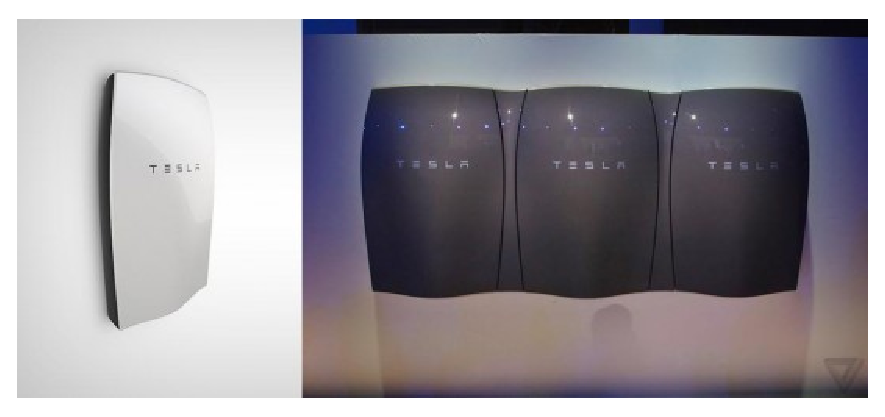
\includegraphics[keepaspectratio,scale=1]{figuras/powerwall.eps}
	\caption{Powerwall\cite{TESLA}}
  \end{center}
\end{figure}

\subsection{Quantidade de baterias necessárias}

	Para o projeto da casa, necessita-se de no máximo 4 baterias, no qual essas já teriam capacidade de alimentar a residência em suas necessidades básicas (como cozinha, iluminação e equipamentos de monitoramento e de segurança), por vários dias no caso de apagão.

\subsection{Especificações de instalação}

	O seu dimensionamento é de 130cmx68cmx18cm para cada uma, e funcionando na faixa de temperatura -20\si{\celsius} a 43\si{\celsius} \cite{TESLA}

	Essas baterias apresentam uma conexão com a internet, onde é possível o monitoramento da energia armazenada e quanto está sendo gasta. Tais baterias quando carregadas e descarregadas entre 20\% e 80\% do seu total de armazenamento, com vida útil de 1500 ciclos, durariam por anos, tendo uma garantia de 10 anos pela empresa \cite{TESLA}.

\subsection{Sistema Grid-Tie}

	Para os painéis solares na casa, serão 12 placas ao todo, tendo duas ligações em série de 6 placas cada. Para esse sistema, tem-se duas opções de instalação dos inversores grid-tie, a modular e a central.

	\textsc{central} - Recebe energia de vários painéis solares, ligados em série e paralelo, estabilizando com um único otimizador MPPT e fazendo sua função de inversor DC/AC. Há um ganho de custo por utilizar menor número de inversores, porém há menor flexibilidade de projeto e manutenção.

	\textsc{modular} - Cada inversor recebe uma série ou string e vários inversores são utilizados em paralelo, cada um com seu otimizador MPPT. Essa configuração permite maior flexibilidade, como diferentes orientações para cada string. Além disso, eventuais perdas com defeitos, sujeiras, sombreamentos, etc. são minimizados pois cada série funciona separadamente.

	Devido à quantidade dos painéis solares, e mantendo-se a manutenção e os devidos cuidados para sempre manter a eficiência em alta com os painéis, o opção pelo sistema central já é capaz de satisfazer as necessidades da família e tendo uma melhor relação entre custo-benefício.

\subsection{Manutenção}

	Tal produto dispensa manutenção desde que suas condições de operação sejam seguidas, tais como estar em ambientes com temperaturas entre -25\si{\celsius} e +50\si{\celsius}, entre outras especificações técnicas. O produto possui garantia de 5 anos e vida útil acima de 10 anos\cite{neosolarKitGerador}.

\subsection{Controle da quantidade gerada e consumida}

	O controle pode ser feito diretamente olhando ao quadro de energia, ou por meio de recebimento de dados, já que os inversores presentes atualmente no mercado possuem sistema de monitoramento integrado à conexão WLAN\cite{neosolarKitGerador}.

\subsection{Quadro comparativo entre modelos grid-tie}

Para o caso proposto, o inversor irá variar entre 2.142 \si{\kilo\watt} e 3.672 \si{\kilo\watt}. O valor adotado para o projeto foi de 0,9P ins , que é 2.754 \si{\kilo\watt}.

Com os dados acima, foi encontrado dois possíveis inversores para o projeto. A seguir, encontra-se uma tabela (\ref{comparaca_inversores}) comparativa entre ambos.

\begin{table}[H]
\centering
\begin{tabular}{|c|c|c|c|c|c|}
\hline 
\textbf{Modelo} & \textbf{Potência} [\si{\watt}] & \textbf{I}\textsubscript{max\_entrada} [\si{\ampere}] & \textbf{V}\textsubscript{max\_entrada} [\si{\volt}] & \textbf{Peso} [\si{\kilo\gram}] & \textbf{Preço} [R\$]\tabularnewline
\hline 
\hline 
Fronius & \multirow{2}{*}{3.100} & \multirow{2}{*}{20,7} & \multirow{2}{*}{165 a 440} & \multirow{2}{*}{16,8} & \multirow{2}{*}{8.090,00}\tabularnewline
Galvo 3.1-1 &  &  &  &  & \tabularnewline
\hline 
Sunny Boy 3300 & \multirow{2}{*}{3.300} & \multirow{2}{*}{20} & \multirow{2}{*}{200 a 400} & \multirow{2}{*}{38} & \multirow{2}{*}{12.790,00}\tabularnewline
03.101.005 &  &  &  &  & \tabularnewline
\hline 
\end{tabular}
\caption{Comparação entre inversores}
\label{comparaca_inversores}
\end{table}

Dentre os modelos apresentados, o que melhor se encaixa ao projeto da casa é o Fronius Galvo 3.1-1 porque ele possui um menor custo, a corrente de entrada é ligeiramente maior e o range de operação da voltage é maior. Uma vez que ele opera com uma voltagem menor do que o Sunny Boy e sua voltagem máxima é maior. E um outro importante ponto é o peso do inverso que é pouco menos da metade do Sunny Boy.

	Com isso, foi feita uma análise para determinar o melhor arranjo do sistema, levando em consideração as características técnicas das placas e do inversor. A corrente máxima que o inversor suporta é 20,7\si{\ampere}(6) . A corrente de curto circuito das placas é 8,89\si{\ampere} e a tensão de circuito aberto é 37,8\si{\volt}(4).

	Para o arranjo em paralelo(2):
	
	$$I_T\ =\ 8,89 + 8,89\ =\ 17,78\si{\ampere}$$
	$$V_T\ =\ 6\times V_{oc}\ =\ 6\times37,8\ =\ 226,8\si{\volt}$$

	Para o arranjo em série(2):
	
	$$I_T\ =\ 8,89\si{\ampere}$$
	$$V_T\ =\ 12\times V_{oc}\ =\ 12\times37,8\ =\ 453,6\si{\volt}$$

	Com os dados acima, foi possível verificar que o melhor arranjo para o sistema é o em paralelo pois a corrente e a tensão estão dentro do range do inversor escolhido. Já o arranjo em série irá extrapolar na tensão do inversor, que suporta no máximo 440\si{\volt} contra 453,6\si{\volt}.

%%%%%%%%%%%%%%%%%%%%%%%%%%%%%%%%%%%%%%%%%%%%%%%%%%%%%%%%%%%%%%%%%%%%%%%%%%%%%%
%%%%%%%%%%%%%%%%%%%%%%%%% Reaproveitamento da água %%%%%%%%%%%%%%%%%%%%%%%%%%%
%%%%%%%%%%%%%%%%%%%%%%%%%%%%%%%%%%%%%%%%%%%%%%%%%%%%%%%%%%%%%%%%%%%%%%%%%%%%%%

\section{Reaproveitamento da água}

\subsection{Consumo de água médio pela família}

	De acordo com a Organização das Nações Unidas, cada pessoa necessita de 3,3 mil litros de água por mês (cerca de 110 litros de água por dia para atender as necessidades de consumo e higiene). No entanto, no Brasil, o consumo por pessoa pode chegar a mais de 200 \nicefrac{litros}{dia}. Atualmente, cada habitante do DF consome, em média, 190 litros diários, de acordo com a Companhia de Saneamento Ambiental do Distrito Federal (Caesb).
	
	Em Brasília o consumo médio por habitante é de 190\nicefrac{litros de água}{dia}, o que resulta em um consumo mensal médio de 6m3 por habitante. Para a casa com 4 habitantes, o consumo mensal médio será de 24\si{\meter}$^3$.

\subsection{Reuso da água}

	Por se tratar de um bem natural que está cada vez mais raro e caro, reutilizar a água é de fundamental importância para o meio ambiente e também para a economia das empresas, cidadãos e governos. Evitar o desperdício é a chave para a preservação.
	
	Será reaproveitada a água cinza que consiste em qualquer água residual, a partir de processos domésticos como lavar louça, roupa e tomar banho. A água cinza corresponde de 50\% a 80\% de esgoto residencial e a água da chuva que será armazenada e desse armazenamento resultará em um aproveitamento de 100\%.

	Já a água da chuva pode muito bem ser utilizada em descargas sanitárias, irrigação de jardins, limpeza de calçada, pátios, paredes, veículos, em espelhos e fontes d’água, sistemas de resfriamentos, entre outros, economizando assim a água tratada, que poderá ser usada apenas para fins mais nobres.

\subsection{Quantidade de água consumida}

	O consumo de água em uma residência é influenciado por diversos fatores, tais como: clima da região, renda familiar, número de habitantes da residência, características culturais da comunidade, desperdício domiciliar, valor da tarifa de água e estrutura e forma de gerenciamento do sistema de abastecimento.

	O cidadão contribuiria com o meio ambiente e com a disponibilidade do recurso para gerações futuras se consumisse 150 litros diários, segundo parâmetros da Agência Reguladora de Águas, Energia e Saneamento do DF (Adasa).

	A média recomendada pela Organização Mundial da Saúde (OMS) é ainda menor. Para assegurar as necessidades básicas e minimizar os problemas de saúde, o órgão estipula uma média diária de 100 litros por habitante. O DF está entre as regiões que mais consomem água no país. Em 2011, segundo dados do Sistema Nacional de Informações sobre o Saneamento (Snis) do Ministério das Cidades, o consumo médio chegava a 187 litros de água diários por habitante, média ultrapassada apenas pelo Rio de Janeiro (237,8), pelo Espírito Santo (192) e pelo Amapá (187,5). Desde então, o DF registrou uma redução, mas, segundo a Caesb, a taxa mantém-se praticamente constante. Atualmente, cada habitante do DF consome, em média, 184 litros diários, de acordo com a Companhia de Saneamento Ambiental do Distrito Federal (Caesb). [1]

	Segundo Hafner (2007) ao se analisar a distribuição do consumo de água em unidades residenciais de vários estudos e trabalhos, verifica-se que os valores são bastante divergentes entre si, mas também é possível perceber algumas tendências gerais. 
	
	O chuveiro e as descargas das bacias sanitárias são os maiores consumidores de água. O terceiro na lista geral de consumo de água é a pia da cozinha, que deve ser analisada junto a máquina de lavar louça, uma vez que nem todos os lares possuem esta segunda peça. Seguindo a ordem dos consumos tem-se a máquina de lavar roupa, o lavatório e o tanque.

\subsection{Finalidade da água não aproveitada}

	A água não aproveitada ou também chamada de água negra, geralmente água do vaso sanitário será descartada na rede de esgoto. O esgoto produzido pela residência será despejado na rede, pois com relação ao índice de atendimento à população, segundo dados do censo demográfico 2010 realizado pelo IBGE, 88,9\% das residências urbanas possuem saneamento adequado e 10,9\% semi-adequado. Esses dados sugerem que o Distrito Federal possui o maior índice de cobertura de saneamento no Brasil, que acaba mostrando que é explicitamente mais viável utilizar a rede pública.

	A empresa responsável pelo tratamento é a CAESB, que possui um nível de tratamento terciário do esgoto, enquanto outras empresas utilizam apenas o tratamento secundário, que é um dos motivos que diferencia as ETE's do DF das demais. O tratamento a nível primário são sedimentados os sólidos em suspensão que vão se acumulando no fundo do decantador, formando o lodo primário que depois é retirado para dar continuidade ao processo. Em seguida, no tratamento a nível secundário, os microrganismos irão se alimentar da matéria orgânica, convertendo-a em gás carbônico e água. E por final, no tratamento a nível terciário são removidos poluentes específicos como micronutrientes (fósforo e nitrogênio) o que garante a qualidade ainda maior do tratamento.
	
	Outra característica importante na escolha do tratamento de esgoto da rede pública é que ao analisarmos o esgotamento sanitário no DF, os lodos de esgoto, em geral, possuem concentrações de substâncias químicas dentro dos limites estabelecidos pela legislação, e desse modo a Caesb incentiva a destinação ambientalmente equilibrada desses lodos por meio de sua incorporação ao solo agricultável, isto é, por meio da reciclagem dos seus nutrientes e matéria orgânica em atividades de agricultura, de silvicultura ou de recuperação de áreas mineradas.

\subsection{Processo de captação da água}

	No processo de captação da chuva, é necessário ter na construção um sistema de captação e armazenamento dessa água. O princípio desses sistemas é simples: a água é captada antes que entre em contato com o solo ou local de trânsito de pessoas, animais e veículos, evitando assim contaminação, através de telhados e calhas que direcionam a água para um filtro autolimpante que irá retirar os resíduos e levá-la diretamente para cisternas (EMBRAPA).

\subsection{Sistema de tratamento da água}

	A cisterna será implementada no quintal da casa ou subsolo com capacidade de 16 mil litros de água, é necessário um acompanhamento periódico da cisterna, assim como o centro de tratamento da água cinza.
	
	O aproveitamento de água de chuva em residências pode contribuir com a conservação de mananciais, com a redução de enchentes nas cidades e com a diminuição da utilização de energia e insumos na captação, adução, tratamento e distribuição de água potável.
	
	A água de chuva armazenada sem tratamento adequado pode ser utilizada apenas para consumo não potável. A água de chuva tem potencial para utilização na descarga de vasos sanitários, lavagem de roupas, irrigação de jardins, na lavagem de carros, em sistemas de ar-condicionado e em sistemas de combate de incêndios, entre outros.
	
	Um sistema de aproveitamento de água de chuva possui, em geral, os seguintes componentes:

\begin{enumerate}
\item \textbf{Área de coleta}: local onde a chuva precipita a fim de ser captada. É importante no dimensionamento do volume de reservação, pois quanto mais for à área de captação maior será o volume de água de chuva capturado e armazenado. A área de captação deve suprir a demanda de consumo de água.

\item \textbf{Calhas e condutores}: Condutos que levam a água captada até o reservatório. As calhas são dispostas na horizontal e os condutos na vertical. Os dimensionamentos desses componentes devem seguir a NBR 10844.

\item \textbf{Dispositivo de descarte das "primeiras águas"}: componente utilizado para descartar a água que lava a área de captação, local onde se acumula poeira, fuligem e outros contaminantes atmosféricos que podem alterar a qualidade da água. Para este descarte pode-se dispor de desvio manual da água ou dispositivos instalados em boias de tanques intermediários.

\item \textbf{Separador de materiais grosseiros}:dispositivo utilizado para a separação de galhos, folhas e outros materiais que podem ser depositados na área de captação. Existem no mercado filtros produzidos para esta função.

\item \textbf{Armazenamento}:sistema composto por dois reservatórios. Um inferior, enterrado com o objetivo armazenar a água coletada e compensar a variação da precipitação de chuva, e um reservatório superior para distribuição por gravidade até os pontos de utilização.

\item \textbf{Sistema de recalque}: composto por bomba, tubulações e conexões. Responsável pelo transporte de água do reservatório inferior para o reservatório superior

\item \textbf{Sistema de distribuição}: responsável pelo abastecimento de água de chuva nos pontos de utilização (ex.: bacias sanitárias). Composto por barrilete, colunas, ramais e sub-ramais de distribuição (TOMAZ, 2003).

\end{enumerate}

\subsection{Dimensionamento}

\subsubsection{Previsão do consumo de água não potável}

Para o dimensionamento do sistema é necessário que primeiramente seja estimado o consumo de água a ser utilizado. Na ausência de dados locais podem ser utilizados dados da literatura, como os dados das tabelas a seguir.

\begin{table}[H]
\centering
\begin{tabular}{|c|c|c|c|}
\hline 
\multicolumn{2}{|c|}{\textbf{Demanda}} & \textbf{Unidade} & \textbf{Faixa}\tabularnewline
\hline 
\hline 
\multicolumn{4}{|c|}{\textbf{Uso interno}}\tabularnewline
\hline 
\multirow{2}{*}{\textbf{Vaso Sanitário}} & Volume & L/descarga & 6 a 15\tabularnewline
\cline{2-4} 
 & Frequência & Descarga/hab/dia & 3 a 6\tabularnewline
\hline 
\multirow{2}{*}{\textbf{Lavagem de roupas}} & Volume & L/ciclo & 108 a 189\tabularnewline
\cline{2-4} 
 & Frequência & Carga/hab/dia & 0,2 a 0,37\tabularnewline
\hline 
\multicolumn{4}{|c|}{\textbf{Uso externo}}\tabularnewline
\hline 
\multirow{2}{*}{\textbf{Gramado ou Jardim}} & Volume & L/dia/m2 & 2\tabularnewline
\cline{2-4} 
 & Frequência & Lavagem/mês & 8 a 12\tabularnewline
\hline 
\multirow{2}{*}{\textbf{Lavagem de Carro}} & Volume & L/lavagem/carro & 80 a 150\tabularnewline
\cline{2-4} 
 & Frequência & Lavagem/mês & 1 a 4\tabularnewline
\hline 
\multirow{2}{*}{\textbf{Lavagem área impermeável}} & Volume & L/lavagem/carro & 80 a 150\tabularnewline
\cline{2-4} 
 & Frequência & Lavagem/mês & 1 a 4\tabularnewline
\hline 
\multicolumn{2}{|c|}{\textbf{Manutenção de piscinas}} & L/dia/m2 & 3\tabularnewline
\hline 
\end{tabular}
\caption{Demanda de água não potável em uma residência\cite{FAdaptado de TOMAZ,2003}}
\label{demanda_de_agua}
\end{table}

\begin{table}[H]
\centering
\begin{tabular}{|c|c|}
\hline 
\textbf{Aparelho/uso} & \textbf{\% do Consumo}\tabularnewline
\hline 
\hline 
\textbf{Descargas nas pacias sanitárias} & 14\% a 41\%\tabularnewline
\hline 
\textbf{Chuveiros e banheiros} & 24\% a 47\%\tabularnewline
\hline 
\textbf{Máquinas de lavar roupas} & 8\% a 9\%\tabularnewline
\hline 
\textbf{Tanque} & 4\% a 18\%\tabularnewline
\hline 
\textbf{Jardins} & 0\% a 3\%\tabularnewline
\hline 
\textbf{Outros} & 0\% a 7\%\tabularnewline
\hline 
\end{tabular}
\caption{Estimativas médias de consumo de água não potável em uma residência}
\label{}
\end{table}

\subsubsection{Volume do reservatório}

Para efeito de cálculo, o volume de água de chuva que pode ser aproveitado não é o mesmo que o precipitado. Para isto usa-se um coeficiente de escoamento superficial chamado de coeficiente de runoff que é o quociente entre a água que escoa superficialmente pelo total da água precipitada. Usa-se a letra C para o coeficiente de runoff, que depende do tipo de superfície, o recomendado é adotar $C\ =\ 0,8$.

	Portanto, a perda de água de chuva que irá ser considerada é devida à limpeza do telhado, perda por evaporação, perdas na autolimpeza e outras.Para determinação do volume do reservatório deve ser calculado o volume precipitado em função de dados meteorológicos de precipitação da região. Para efeito de cálculo, o volume de água que pode ser aproveitado não é o mesmo que o precipitado.
	
	O volume captado por uma superfície é dado pela expressão:
$$V_c = A\times P\times C$$
Onde:
$V_c$ = volume mensal ou anual captado (\si{\liter})
$A$ = área de contribuição ($\si{\meter}^{2}$)
$P$ = precipitação média mensal ou anual (\si{\milli\meter})
$C$ = coeficiente de escoamento

	O volume mínimo de água necessário ($V_{mín}$) deve ser menor ou igual ao volume
captado ($V_c$) para atender a demanda de água

\subsection{Sistema de captação da água da chuva}

	Definição dos sistemas de tratamento, armazenamento e cuidados com a água
coletada. Neste item são definidos os equipamentos de filtragem pré-reservação, onde são removidos todos os elementos que são passiveis de degradação da água depois de reservada numa \uline{cisterna} (Reservatório destinado ao armazenamento da água de chuva coletada), a qualidade e tipo de reservatório a ser utilizado bem como sistemas de tratamento pré-consumo, instalados na saída da cisterna antes dos pontos de consumo, sistemas como: \uline{filtro de areia}, \uline{sistemas de desinfecção}, \uline{Sistema de bombeamento}, etc.

\begin{figure}[H]
\centering
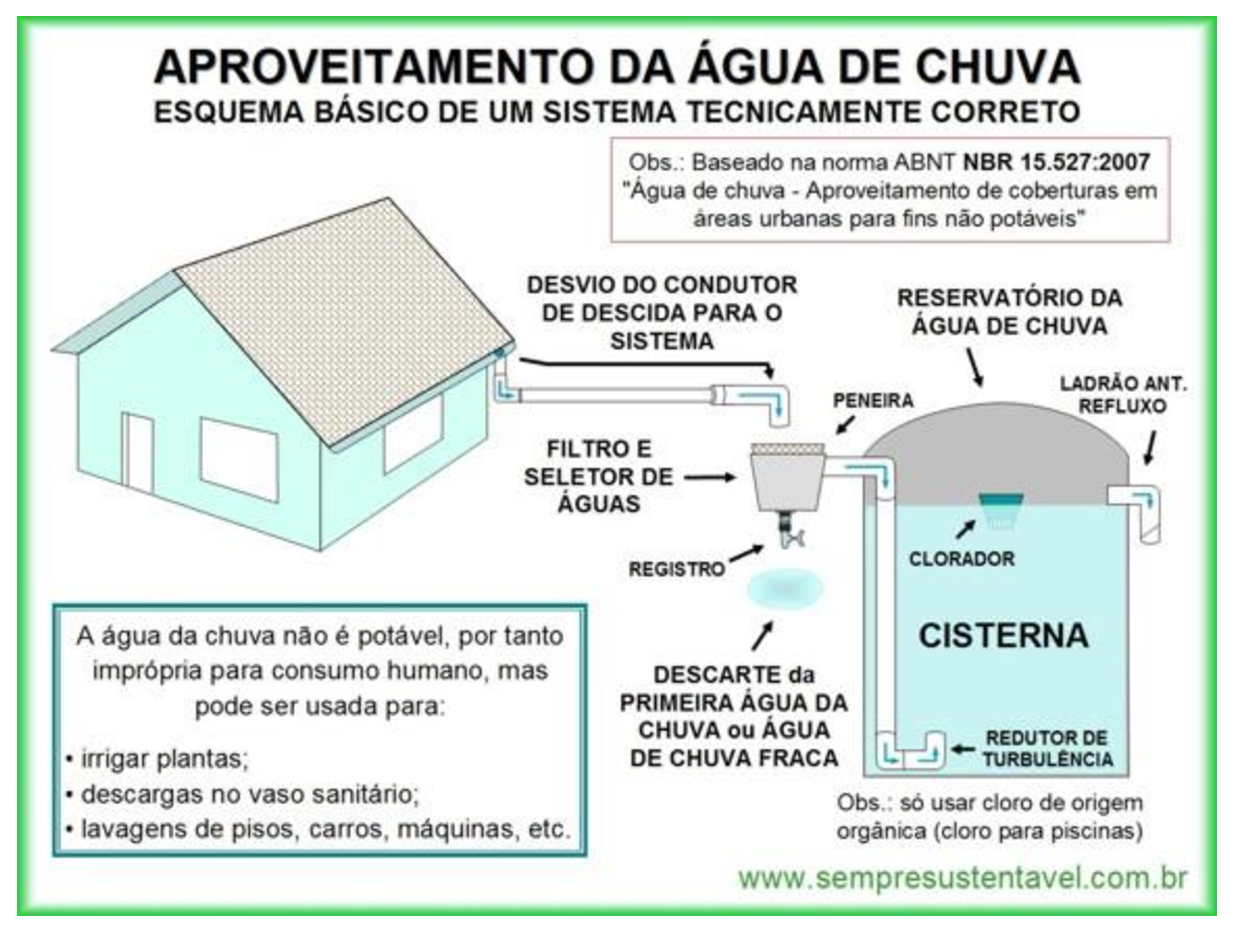
\includegraphics[keepaspectratio,scale=0.6]{figuras/aproveitamento_chuva.eps}
\caption{Aproveitamento da água da chuva}
\end{figure}

\subsubsection{Reservatórios ou cisternas}
\begin{itemize}
\item Os reservatórios ou cisternas podem ser: enterrados, semienterrados, poiado ou elevado. Os materiais podem ser concreto, alvenaria armada, materiais plásticos como polietileno, PVC, fibra de vidro e aço inox. Sempre serão vedados a luz solar.

\item Os reservatórios devem ser construídos como se fosse para armazenamento de água potável devendo serem tomadas os devidos cuidados para não contaminar a água de chuva coletada dos telhados.

\item Devem ser considerados no projeto do reservatório: extravasor, descarga de fundo ou bombeamento para limpeza, cobertura, inspeção, ventilação e segurança.

\item O reservatório quando alimentado com água de outra fonte de suprimento de água, deve possuir dispositivos que impeçam a \textit{conexão cruzada}.

\item O volume de água de chuva aproveitável depende do coeficiente de runoff, bem como da eficiência do sistema de descarte do \textit{first flush}, sendo calculado pela seguinte equação:

$$V\ =\ P\times A\times C\times N$$

Onde:
$V$ = Volume anual, mensal ou diário de água de chuva aproveitável
$P$ = Precipitação média anual, mensal ou diária;
$A$ = Área de coleta;
$C$ = Coeficiente de escoamento superficial da cobertura;
$N$ = Fator de captação é a eficiência do sistema de captação, levando em conta o dispositivo de descarte de sólidos e desvio de escoamento inicial, caso este último seja utilizado

\end{itemize}

\subsubsection{Calhas e condutores}

	As calhas e condutores horizontais e verticais devem atender a ABNT NBR 10844/89 sendo que tais dimensionamento são baseados em vazões de projeto que dependem dos fatores meteorológicos e do período de retorno escolhido. Estas vazões não servem para dimensionamento dos reservatórios e sim para o dimensionamento das calhas e condutores (verticais e horizontais). 

	Devem ser observados o período de retorno escolhido (T$_{r}$), a vazão de projeto e a intensidade pluviométrica. Recomenda-se T$_{r}$ = 25 anos. Nos condutores verticais ou nos condutores horizontais pode ser instalado dispositivos fabricados ou construídos in loco para o descarte da água do \textit{first flush} ou para eliminação de folhas e detritos. O dispositivo ou a construção poderá ter operação manual ou automática sendo recomendado a operação automática. O dispositivo de descarte de água do \textit{first flush} deve ser dimensionado pelo projetista. Na falta de dados recomenda-se no mínimo 2 \si{\milli\meter}, ou seja, 2 \nicefrac{litros}{$\si{\meter}^{2}$} de telhado.

	Caso se julgue conveniente poderão ser instaladas telas ou grades para remoção dedetritos.Vazão na calha
Conforme NBR 10844/89 a vazão na calha é dada pela equação:

\subsubsection{Vazão na calha}

	Conforme NBR 10844/89 a vazão na calha é dada pela equação:

$$Q\ =\ \dfrac{I\times A}{60}$$

	Sendo:
$Q$= vazão de pico (\nicefrac{litros}{min})
$I$= intensidade pluviométrica (\nicefrac{\si{\milli\meter}}{\si{\hour}})
$A$= area de contribuição ($\si{\meter}^{2}$)

Os períodos de retorno comumente adotado é T$_{r}$ = 25 anos para cidades acima de 100.000 habitantes (Ilha de Calor). Para a RMSP adotamos o mínimo: I = \nicefrac{200\si{\milli\meter}}{\si{\hour}}.

\subsubsection{Dimensionamento da calha}

É usado para dimensionamento da calha a fórmula de Manning:

$$Q\ =\ 60000\times \dfrac{A}{n}\times R_{(2/3)} \times S_{0,5}$$

Sendo:
$Q$= vazão de pico (\nicefrac{L}{min})
$A$= área da seção molhada ($\si{\meter}^{2}$)
$n$= coeficiente de rugosidade de Manning. Para concreto $n$=0,013 e para plástico $n$=0,011.
$R$= raio hidráulico= \nicefrac{A}{P}
$P$= perímetro molhado (\si{\meter})
$S$= declividade da calha (\nicefrac{\si{\meter}}{\si{\meter}})

\begin{table}[H]
\centering
\begin{sideways}
\begin{tabular}{|c|c|c|c|c|c|c|c|c|c|}
\hline 
\multirow{3}{*}{Diâmetro do} &  & \multicolumn{4}{c|}{Capacidade dos condutores horizontais (Calhas)} &  & \multicolumn{3}{c|}{Capacidade dos condutores verticais}\tabularnewline
 &  & \multicolumn{4}{c|}{e seção circular (formato) com} &  & \multicolumn{3}{c|}{(tubos de descida da água das calhas)}\tabularnewline
 &  & \multicolumn{4}{c|}{Vazões em \nicefrac{litros}{minuto}} &  & \multicolumn{3}{c|}{}\tabularnewline
\cline{1-1} \cline{3-6} \cline{8-10} 
\multirow{4}{*}{Tubo D (\si{\milli\meter})} &  & \multicolumn{4}{c|}{Tipo de material = plástico, } &  & \multirow{2}{*}{Vazão} & \multicolumn{2}{c|}{Área do}\tabularnewline
 &  & \multicolumn{4}{c|}{fibrocimento, aço, metais não ferrosos} &  &  & \multicolumn{2}{c|}{telhado}\tabularnewline
\cline{3-6} \cline{8-10} 
 &  & Inclinação 0.5\%  & Inclinação 1\%  & Inclinação 2\%  & Inclinação 4\%  &  & \multirow{2}{*}{\nicefrac{litros}{segundo}} & Chuva muito & Chuva forte\tabularnewline
 &  & (0.5\nicefrac{\si{\centi\meter}}{\si{\meter}}) & (1\nicefrac{\si{\centi\meter}}{\si{\meter}}) & (2\nicefrac{\si{\centi\meter}}{\si{\meter}}) & (4\nicefrac{\si{\centi\meter}}{\si{\meter}}) &  &  & forte 150 \nicefrac{\si{\milli\meter}}{\si{\hour}} & 120 \nicefrac{\si{\milli\meter}}{\si{\hour}}\tabularnewline
\cline{1-1} \cline{3-6} \cline{8-10} 
50 &  & 32 & 45 & 64 & 90 &  & 0.57 & 14 & 17\tabularnewline
\cline{1-1} \cline{3-6} \cline{8-10} 
75 &  & 95 & 133 & 188 & 267 &  & 1.76 & 42 & 53\tabularnewline
\cline{1-1} \cline{3-6} \cline{8-10} 
100 &  & 204 & 287 & 405 & 575 &  & 3.78 & 90 & 114\tabularnewline
\cline{1-1} \cline{3-6} \cline{8-10} 
125 &  & 370 & 521 & 735 & 1.040 &  & 7.00 & 167 & 212\tabularnewline
\cline{1-1} \cline{3-6} \cline{8-10} 
150 &  & 602 & 847 & 1.190 & 1.690 &  & 11.53 & 275 & 348\tabularnewline
\cline{1-1} \cline{3-6} \cline{8-10} 
200 &  & 1.300 & 1.820 & 2.570 & 3.650 &  & 25.18 & 600 & 760\tabularnewline
\hline 
\end{tabular}
\end{sideways}
\caption{Tabela de dimensionamento das calhas e tubos de descidas}
\end{table}
Obs: os dados foram baseados na norma NBR 10844/89 instalações prediais de águas pluviais ABNT







\section{(Re)utilização do lixo doméstico}

\subsection{Lixo produzido}

No Brasil, são coletados aproximadamente 173.583 de toneladas de lixo por dia de acordo com o Panorama de resíduos sólidos no Brasil realizado pela Associação de Empresas de Limpeza (ABRELPE) em 2010. Sendo que 99.919t/d (57,6\%) são destinados a aterros sanitários, 42.231 (24,3\%) vão para aterros controlados que, segundo a NBR 8849/1985 da ABNT, é uma técnica de disposição de resíduos sólidosurbanos no solo, que consiste na cobertura desses resíduos com uma camada de material afim de confiná-lo. E o restante de 31.433 t/dia (18,1\%) é distribuído em lixões.

No Distrito Federal, são coletados diariamente 3.951t/dia de lixo, sendo 1,596kg produzido por cada habitante diariamente, o que torna Brasília a maior produtora de lixo por habitante do Brasil e a maior parte deste, é destinado a aterros controlados, com base em informações da Abrelpe. Tomando como base a média regional, a quantidade de moradores da residência, a quantidade de resíduos sólidos produzidos diariamente na casa, sendo eles ecicláveis e orgânicos, é de 6,384 kg/hab/dia.

\subsection{Classificação dos resíduos produzidos}

Com base no estudo do Instituo GEA e no Instituto de Biociências da USP acerca da classificação de matérias recicláveis e seu devido descarte, onde a tabela abaixo identifica os resíduos mais comuns produzidos por uma família e o seu descarte adequado.

\newpage

\begin{table}[H]
\centering
\begin{tabular}{|c|c|c|c|}
\hline 
Resíduos produzidos & Coleta seletiva & Compostagem & Outros\tabularnewline
\hline 
\hline 
Papel & x &  & \tabularnewline
\hline 
Plástico & x &  & \tabularnewline
\hline 
Metal & x &  & \tabularnewline
\hline 
Vidro & x &  & \tabularnewline
\hline 
Madeira &  &  & \tabularnewline
\hline 
Carnes e peixes &  & x & \tabularnewline
\hline 
Massas e grãos &  & x & \tabularnewline
\hline 
Verduras e frutas &  & x & \tabularnewline
\hline 
Tecidos & x &  & \tabularnewline
\hline 
Cigarros &  &  & x\tabularnewline
\hline 
Produtos eletrônicos & x &  & \tabularnewline
\hline 
Medicamentos & x &  & \tabularnewline
\hline 
Outros alimentos &  & x & \tabularnewline
\hline 
Papel higiênico & \multirow{2}{*}{} & \multirow{2}{*}{} & \multirow{2}{*}{x}\tabularnewline
Papel toalha &  &  & \tabularnewline
\hline 
Absorventes & \multirow{3}{*}{} & \multirow{3}{*}{} & \multirow{3}{*}{x}\tabularnewline
Preservativos &  &  & \tabularnewline
Fraldas &  &  & \tabularnewline
\hline 
\end{tabular}
\caption{Resíduos produzidos e destinação}
\end{table}

\subsection{Quantidade de resíduos produzidos}

Com base nos dados coletados, obtém-se os resultados da quantidade de lixo produzido e a sua reutilização através de um quadro comparativo, considerando que toda a família produza cerca de 6,384 kg/hab/dia.

\begin{table}[H]
\centering
\begin{tabular}{|c|c|c|c|}
\hline 
Tipo de & \multirow{2}{*}{Destinação} & Porcentagem do tipo de & Quantidade em\tabularnewline
Resíduo &  & resíduo produzido/dia & kg/hab/dia\tabularnewline
\hline 
\hline 
Seco & Coleta Seletiva & 60\% & 3;830\tabularnewline
\hline 
Orgânico & Compostagem & 35\% & 2.234\tabularnewline
\hline 
Outros & Lixo comum & 5\% & 0.320\tabularnewline
\hline 
\end{tabular}
\caption{Destinação e quantidade de lixo produzido}
\end{table}

	A tabela expressa o tipo de resíduo produzido, a destinação e a quantidade do mesmo. Como destinação do lixo seco, a coleta seletiva é o mais adequado pois através dela é possível separar os produtos que são recicláveis. Já a compostagem é a mais adequada para o lixo orgânico, pois através dela consegue reaproveitar o que seria despejado na natureza produzindo adubo. Já os resíduos que não se encaixam como lixo seco ou orgânico (não são aproveitados nem para compostagem e nem para coleta seletiva), serão destinados ao lixo comum, no qual se refere ao lixo coletado por uma empresa responsável e destinado a aterros.

	Através da seguinte estimativa, conclui-se que quase cem por cento do lixo pode ser reaproveitado, caso o descarte seja feito de maneira adequada pelos moradores da residência.

	Logo abaixo podemos visualizar a tabela da disposição diária e mensal de geração de resíduos por morador e o total da produção pela quantidade de moradores na residência.

\begin{table}[H]
\centering
\begin{tabular}{|c|c|c|c|}
\hline 
Tipo de & \multicolumn{1}{c|}{Produção diária de} & Produção mensal de & Produção mensal de\tabularnewline
Resíduo & resíduos por morador & resíduo por morador & resíduos - 4 moradores\tabularnewline
\hline 
\hline 
Seco & 0,957 & 28,71 & 114,84\tabularnewline
\hline 
Orgânico & 0,559 & 16,77 & 67,08\tabularnewline
\hline 
Outros & 0,08 & 2,4 & 9,6\tabularnewline
\hline 
Total & 1,596 & 47,88 & 191,52\tabularnewline
\hline 
\end{tabular}
\caption{Produção diária e mensal de resíduos da residência}
\end{table}

Na seguinte tabela podemos observar a relação entre a quantidade de lixo produzido pela residência e a quantidade que irá ser reaproveitada.


\begin{table}[H]
\centering
\begin{tabular}{|c|c|c|c|}
\hline 
Tipo de & \multicolumn{1}{c|}{Produção mensal de} & \multirow{2}{*}{Destinação} & Quantidade total re-\tabularnewline
Resíduo & resíduos - 4 moradores &  & aproveitada por mês\tabularnewline
\hline 
\hline 
Seco & 114,84 & Coleta Seletiva & 114,84\tabularnewline
\hline 
Orgânico & 67,08 & Composteira & 67,08\tabularnewline
\hline 
Outros & 9,6 & Lixo comum & -\tabularnewline
\hline 
Total & 191,52 & - & 181,92\tabularnewline
\hline 
\end{tabular}
\caption{Relação da quantidade de resíduos descartados e reaproveitados}
\end{table}

Como podemos observar, a quantidade de resíduos produzidos por mês pela residência com quatro habitantes tomando como base a média do Distrito Federal, é de 191,52kg. E a importância do descarte adequado do lixo da residência utilizando coleta seletiva e a composteira, representa uma diferença de aproximadamente 181,92kg de lixos que não serãodestinados a aterros ou despejados na natureza de forma incorreta e que possam degradar mais ainda o meio ambiente.

\subsection{Lixo destinado ao serviço de limpeza urbana}

O Distrito Federal tem os serviços de saneamento prestados pela Companhia de
Saneamento Ambiental do DF/Caesb (água e esgoto), pela Companhia Urbanizadora da Nova Capital do Brasil/Novacap (drenagem urbana) e pelo Serviço de Limpeza Urbana/SLU (limpeza urbana e manejo dos resíduos sólidos).

Com base no Relatório de Diagnósticos de Resíduos Sólidos realizado pelo Sistema de Limpeza Urbano do DF, a quantidade de lixo coletado seletivamente pelo SLU, chega a 9,88\% em toda a região, mas considerando rejeitos, apenas 2\% desse total foram encaminhados à reciclagem. Do total de lixo coletado no Jardim Botânico, cerca de 60\% dele faz parte da coleta seletiva.

De acordo com a população do Distrito Federal e a quantidade de lixo coletado, é possível estimar que cerca de 60\% do lixo sólido gerado pela residência é seco e será destinado a coleta seletiva para reciclagem desses materiais. Pois no Jardim Botânico a coleta realizada pelo SLU é realmente efetiva.

\subsection{Detalhamento do processo de separação do lixo}

A reciclagem reduz o impacto sobre o meio ambiente, gera economia de água e luz.
Diminui as retiradas de matéria-prima da natureza e a disposição inadequada do lixo. Para o
processo de separação do lixo residencial, será utilizada a prática dos 3 R's que é: reduzir, reciclar
e reutilizar.

O processo de separação dos resíduos sólidos da residência será feito manualmente
pelos integrantes da família. Primeiramente, é necessário que a pessoa que faça a separação
conheça e saiba diferenciar o lixo reciclável (papel, jornais, garrafas plásticas, recipientes de
limpeza, latinhas de alumínio, embalagens e produtos eletroeletrônicos e entre outros) do lixo
orgânico (cascas de frutas e legumes, sobras de alimento).

Após a identificação de cada tipo de material, é necessário que o lixo reciclável seja
limpo, seco e armazenado separadamente do lixo orgânico, para que possa ser entregue a
coleta seletiva da região feita pelo SLU. Já o lixo orgânico será separado manualmente para a
utilização na composteira doméstica.

\subsection{Detalhamento do processo de reutilização do lixo orgânico}

Visando as necessidades de se descartar o lixo orgânico corretamente, a residência terá
uma composteira, que é basicamente um processo de decomposição e de reciclagem de matéria
orgânica contida em restos de origem animal ou vegetal, formando um composto rico em
substâncias húmicas e nutrientes que podem ser como adubo na manutenção do jardim.

Na escolha do modelo mais adequado para a residência, foi escolhido uma composteira
automática que é movida a energia elétrica e acaba se tornando um método mais prático e
simples de se fazer a compostagem. As vantagens na utilização desse tipo de composteira aoinvés da convencional, é pelo fato de que ela pode ser instalada em praticamente qualquer
espaço da casa, não requer muito conhecimento para manuseio do aparelho, não traz
problemas com odores. Outro fator relevante é o tempo que ela leva para compostar o alimento,
que é de 24h ao contrário das convencionais que podem levar até 60 dias.

A composteira elétrica funciona diferentemente da convencional que possui minhocas
no seu processo. Nela se faz o uso de poderosos microrganismos patenteados capazes de se
multiplicarem em altas temperaturas, acidez, salinidade e que possuem uma alta longevidade
o que torna a manutenção sem custos adicionais.

\subsection{Comparativo dos modelos de composteira}

Para o reaproveitamento do lixo orgânico da residência, conforme apresentado no
quadro comparativo para verificar quais tipos de recursos para a destinação desses resíduos, e
através dos resultados justificar a escolha pela utilização da composteira elétrica no processo de
reutilização.

\begin{table}[H]
\centering
\begin{tabular}{|c|c|c|}
\hline 
Reaproveitamento & Compostagem comum & Compostagem elétrica\tabularnewline
\multirow{2}{*}{do lixo orgânico} & Composteira doméstica kit GG & \multirow{2}{*}{Decomposer2}\tabularnewline
 & + Minhocas californianas & \tabularnewline
\hline 
Custo (R\$) & 415,00 & 4299,00\tabularnewline
\hline 
\multirow{2}{*}{Custos adicionais} & Minhocas (300 unidades) & Serragem (1kg) - R\$10,00\tabularnewline
 &  R\$ 60,00 & + Assistência técnica R\$ ?\tabularnewline
\hline 
\multirow{3}{*}{Instalação} & Feita pelo próprio & Feita pelo próprio\tabularnewline
 & consumidor e instalada & consumidor e instalada em\tabularnewline
 & na parte externa da casa & qualquer espaço da casa\tabularnewline
\hline 
Produção do adubo (tempo) & 30-60 dias & 24h\tabularnewline
\hline 
\multirow{3}{*}{Manutenção} & Feita pelo próprio morador & Feita pelo próprio morador e\tabularnewline
\cline{2-3} 
 & Controle de umidade e temp. & de um técnico especializado\tabularnewline
\cline{2-3} 
 & (Sempre que necessário) & caso haja problemas na máquina\tabularnewline
\hline 
Tamanho/capacidade & 62cm x 39cm x 80cm & 40x40cm/78cm de altura\tabularnewline
suportada & Capacidade de até 2 litros & Capacidade de até 5,5kg\tabularnewline
\hline 
\end{tabular}\caption{Especificações compostagem comum e elétrica}
\end{table}

	Em relação a garantia, não é informado pelo fabricante a garantia da composteira
comum, já a elétrica possui assistência de um ano e o valor da Assistência técnica varia de acordo
com a necessidade do usuário, podendo ser ela de instalação, manutenção preventiva ou
corretiva. E em relação a manutenção da composteira comum, o fabricante envia ao usuário um
manual detalhado de utilização juntamente com o produto.

	Além da maior praticidade na hora do manuseio e menor tempo para produção de
adubo, outro fator importante na hora da decisão foi a variedade de alimentos que pode serutilizada nesse tipo de composteira, pois a compostagem comum feita por minhocas, não
processa todo tipo de matéria orgânica (como frutas ácidas e carnes, por exemplo), o que faz
dessa escolha a mais apropriada apesar do custo do aparelho.


\subsection{Especificações da composteira}

O modelo de composteira escolhida para a residência é o Decomposer 2, que possui
40x40cm de comprimento e 78cm de altura, pesa 21kg e consome cerca de 60-80kWh/mês, e
tem capacidade diária de compostagem de aproximadamente 5,5kg de resíduos orgânicos o que
é adequado para uma família de 4 pessoas. A máquina possui três funções que é a de agitação,
calor e fluxo de ar, o que torna o processo muito simples.

A composteira deverá ser alocada na área de serviço ou distante de locais quentes, por
motivos de segurança, já que durante o processo há a emissão de gases metano (CH4), que
podem colocar a família em risco caso esses gases entrem em contato com regiões em alta
temperatura. Para ser utilizada, basta apenas que a pessoa despeje o lixo orgânico dentro da
composteira e ligue o aparelho. Deve-se apenas inserir dentro do tanque de decomposição os
materiais orgânicos que podem ser processados, como restos de comida, frutas, legumes, cascas
de ovo, espinhas de peixes e carnes, apensas tomando cuidado de cortar os resíduos volumosos
em pequenos pedaços para não danificar o aparelho.

Normalmente, a máquina de compostagem processa alimentos cozidos muito mais
rapidamente, em 10 a 12 horas, para completar o ciclo. O tempo de ciclo será mais longo para
resíduos de alimentos crus, como casca de ovo, carnes, peixes, aves e crustáceos. Quanto mais
resíduos crus forem despejados no aparelho, mais longo será o ciclo de compostagem,
especialmente se esses resíduos forem de carne vermelha e de aves.
Após a remoção do composto da máquina, recomenda-se misturar na proporção 1:10 com
terra para que o adubo fique estabilizado. Caso o composto não seja misturado com terra,
esse deve ser utilizado numa quantidade pequena cuja camada seja de 2cm.


\section{Viabilidade econômica}

\begin{table}[H]
\centering
\begin{tabular}{|c|c|c|}
\hline 
Item & Preço unitário (R\$) & Valor Total (R\$)\tabularnewline
\hline 
\hline 
12 Placas & \multirow{2}{*}{1.400,00} & \multirow{2}{*}{16.800,00}\tabularnewline
Mitsubishsi 255W &  & \tabularnewline
\hline 
2 Inversores  & \multirow{2}{*}{8.090,00} & \multirow{2}{*}{16.180,00}\tabularnewline
\cline{1-1} 
Fronius Galvo 3.101 &  & \tabularnewline
\hline 
Instalação e Montagem & 5.000,00 & 5.000,00\tabularnewline
\hline 
\multicolumn{3}{|c|}{\textbf{Valor Total: R\$ 37.980,00}}\tabularnewline
\hline 
\end{tabular}
\caption{Precificação dos componentes, da instalação e montagem}
\end{table}

Como foi calculado anteriormente, as 12 placas irão produzir 400,86kWh/mês e isso em 1 ano é igual a 4,81 MWh. Ao longo dos 35 anos 3 , que é a vida útil das placas, a energia produzida
será 168,36 MWh. O custo da energia solar pode ser calculado entre a razão do valor total da
instalação e a energia gerada(2).

$$\dfrac{37.980,00 [R\$]}{168,36 [\si{\mega\watt\hour}]}\ =\ 225,59 \nicefrac{R\$}{\si{\mega\watt\hour}}$$

De acordo com RIBEIRO e PICARELLI, o custo da energia elétrica da distribuidora é de
568,47 R\$/MWh em Maio de 2015. Isto demonstra que o custo da energia fotovoltaica é
competitiva com o mercado já que ela é quase a metade da tarifa da distribuidora.

\subsection{Payback simples}
Para o cálculo do payback simples foi utilizado o valor da tarifa atual da energia da
distribuidora, CEB, do mês de Maio foi 0,56847 R\$/kWh 2 . O valor economizado por mês será:

$$X_{eco}\ =\ 400,86\times0,56847\ =\ R\$ 227,87/mês$$

O consumo médio da casa é 500kWh/mês, como 100 kWh é a taxa de disponibilidade
no qual o consumidor é obrigado a pagar. Esta taxa é de 100 vezes o valor do kWh aplicado
(RIBEIRO e PICARELLI, 2015). No caso atual, esta taxa possui o valor de R\$56, 85. Logo, o valor
total gasto na casa sem o sistema fotovoltaico é:

$$X_T\ =\ 500\times0,56847\ =\ R\$284,23$$

Como a taxa de disponibilidade é R\$56,85, o valor a ser economizado é R\$227,38. Desta
forma, as placas irão economizar todo mês R\$227,87. O retorno do investimento inicial será
recebido em:

$$Payback\ =\ \dfrac{37.980,00}{227,87}\ =\ 166,67$$ meses ou 14 anos

Como o sistemas terá vida útil de 35 anos, o payback de 14 anos é vantajoso para o
consumidor pois ele irá economizar com eletricidade por um período de aproximadamente 20
anos.

Quanto ao aerogerador escolhido para utilizar no projeto foi o Air 40. O seu valor atualmente é
R\$ 5.800,00 1 . A sua garantia é de 5 anos. De acordo com a professora Petrocchi, a estimativa do
custo de instalação foi feito em 100\% em cima do valor do aerogerador. Desta forma, o custo
total da compra e instalação do aerogerador será:


$$Custo\ =\ 5.800 + 5.800\ =\ R\$ 11.600,00$$

A velocidade média do vento em Brasília é 3.5\nicefrac{\si{\meter}}{\si{\second}} e de acordo com as especificiações técnicas
do aerogerador, este irá produzir cerca de 15\nicefrac{\si{\kilo\watt\hour}}{mês}. Considerando uma eficiência do sistema
de 85\%, a energia gerada será de 12,75 \nicefrac{\si{\kilo\watt\hour}}{mês}.

O preço da energia é 0,56847 \nicefrac{R\$}{\si{\kilo\watt\hour}}. O valor economizado com o aerogerador será:

$$X_{eco}\ =\ 0,56847\times12,75\ =\ R\$7,25 por mês$$

A economia gerada pela fonte eólica não é economicamente viável para o projeto da casa uma
vez que o aerogerador tem garantia de 5 anos. E a economia que ele trará para a casa será
inferior a R\$10 por mês. Isso demonstra que a implantação desta fonte alternativa na região de
Brasília nos dias atuais não é possível devido à baixa incidência da velocidade do vento, que é
de aproximadamente 3,5 \nicefrac{\si{\meter}}{\si{\second}}.

O payback de retorno desta fonte será:

$$\dfrac{R\$ 11.600,00}{R\$ 7,25}\ =\ 1.600$$ meses ou 133 anos.

O retorno de um aerogerador será de 133 anos, o que demonstra que a utilização é
inviável da fonte uma vez que será necessário mais de um aerogerador para o período
necessitado.

Para a aquisição dos painéis solares, baterias, sistema grid-tie, captação de água da
chuva e reutilização das águas cinzas em outros setores da casa, deverá ser feito um
investimento aproximadamente de R\$ 116.000,00.

\begin{table}[H]
\centering
\begin{tabular}{|l|r|r|}
\cline{2-3} 
\multicolumn{1}{l|}{} & \textbf{Investimento Mensal} & \textbf{Investimento Imediato}\tabularnewline
\hline 
\textbf{Conta de Luz} & R\$ 43,67 & \tabularnewline
\hline 
\textbf{Painéis Solares} &  & R\$ 16.800,00\tabularnewline
\hline 
\textbf{Montagem} &  & R\$ 5.000,00\tabularnewline
\hline 
\textbf{Inversores Grid-Tie} &  & R\$ 16.180,00\tabularnewline
\hline 
\textbf{Stringbox} &  & R\$ 1.519,00\tabularnewline
\hline 
\textbf{Aerogerador} &  & R\$ 11.600,00\tabularnewline
\hline 
\textbf{Baterias TESLA} &  & R\$ 53.480,00\tabularnewline
\hline 
\textbf{Sistema de água} &  & R\$ 6.838,00\tabularnewline
\hline 
\textbf{Biodigestor} &  & R\$ 4.300,00\tabularnewline
\hline 
\textbf{Total} & R\$ 43,67 & R\$ 115.717,00\tabularnewline
\hline 
\end{tabular}
\caption{Tabela de investimento}
\end{table}








